\documentclass[]{article}
\usepackage{lmodern}
\usepackage{amssymb,amsmath}
\usepackage{ifxetex,ifluatex}
\usepackage{fixltx2e} % provides \textsubscript
\ifnum 0\ifxetex 1\fi\ifluatex 1\fi=0 % if pdftex
  \usepackage[T1]{fontenc}
  \usepackage[utf8]{inputenc}
\else % if luatex or xelatex
  \ifxetex
    \usepackage{mathspec}
  \else
    \usepackage{fontspec}
  \fi
  \defaultfontfeatures{Ligatures=TeX,Scale=MatchLowercase}
\fi
% use upquote if available, for straight quotes in verbatim environments
\IfFileExists{upquote.sty}{\usepackage{upquote}}{}
% use microtype if available
\IfFileExists{microtype.sty}{%
\usepackage{microtype}
\UseMicrotypeSet[protrusion]{basicmath} % disable protrusion for tt fonts
}{}
\usepackage[margin=1in]{geometry}
\usepackage{hyperref}
\hypersetup{unicode=true,
            pdftitle={capstone\_project},
            pdfauthor={becker},
            pdfborder={0 0 0},
            breaklinks=true}
\urlstyle{same}  % don't use monospace font for urls
\usepackage{color}
\usepackage{fancyvrb}
\newcommand{\VerbBar}{|}
\newcommand{\VERB}{\Verb[commandchars=\\\{\}]}
\DefineVerbatimEnvironment{Highlighting}{Verbatim}{commandchars=\\\{\}}
% Add ',fontsize=\small' for more characters per line
\usepackage{framed}
\definecolor{shadecolor}{RGB}{248,248,248}
\newenvironment{Shaded}{\begin{snugshade}}{\end{snugshade}}
\newcommand{\KeywordTok}[1]{\textcolor[rgb]{0.13,0.29,0.53}{\textbf{#1}}}
\newcommand{\DataTypeTok}[1]{\textcolor[rgb]{0.13,0.29,0.53}{#1}}
\newcommand{\DecValTok}[1]{\textcolor[rgb]{0.00,0.00,0.81}{#1}}
\newcommand{\BaseNTok}[1]{\textcolor[rgb]{0.00,0.00,0.81}{#1}}
\newcommand{\FloatTok}[1]{\textcolor[rgb]{0.00,0.00,0.81}{#1}}
\newcommand{\ConstantTok}[1]{\textcolor[rgb]{0.00,0.00,0.00}{#1}}
\newcommand{\CharTok}[1]{\textcolor[rgb]{0.31,0.60,0.02}{#1}}
\newcommand{\SpecialCharTok}[1]{\textcolor[rgb]{0.00,0.00,0.00}{#1}}
\newcommand{\StringTok}[1]{\textcolor[rgb]{0.31,0.60,0.02}{#1}}
\newcommand{\VerbatimStringTok}[1]{\textcolor[rgb]{0.31,0.60,0.02}{#1}}
\newcommand{\SpecialStringTok}[1]{\textcolor[rgb]{0.31,0.60,0.02}{#1}}
\newcommand{\ImportTok}[1]{#1}
\newcommand{\CommentTok}[1]{\textcolor[rgb]{0.56,0.35,0.01}{\textit{#1}}}
\newcommand{\DocumentationTok}[1]{\textcolor[rgb]{0.56,0.35,0.01}{\textbf{\textit{#1}}}}
\newcommand{\AnnotationTok}[1]{\textcolor[rgb]{0.56,0.35,0.01}{\textbf{\textit{#1}}}}
\newcommand{\CommentVarTok}[1]{\textcolor[rgb]{0.56,0.35,0.01}{\textbf{\textit{#1}}}}
\newcommand{\OtherTok}[1]{\textcolor[rgb]{0.56,0.35,0.01}{#1}}
\newcommand{\FunctionTok}[1]{\textcolor[rgb]{0.00,0.00,0.00}{#1}}
\newcommand{\VariableTok}[1]{\textcolor[rgb]{0.00,0.00,0.00}{#1}}
\newcommand{\ControlFlowTok}[1]{\textcolor[rgb]{0.13,0.29,0.53}{\textbf{#1}}}
\newcommand{\OperatorTok}[1]{\textcolor[rgb]{0.81,0.36,0.00}{\textbf{#1}}}
\newcommand{\BuiltInTok}[1]{#1}
\newcommand{\ExtensionTok}[1]{#1}
\newcommand{\PreprocessorTok}[1]{\textcolor[rgb]{0.56,0.35,0.01}{\textit{#1}}}
\newcommand{\AttributeTok}[1]{\textcolor[rgb]{0.77,0.63,0.00}{#1}}
\newcommand{\RegionMarkerTok}[1]{#1}
\newcommand{\InformationTok}[1]{\textcolor[rgb]{0.56,0.35,0.01}{\textbf{\textit{#1}}}}
\newcommand{\WarningTok}[1]{\textcolor[rgb]{0.56,0.35,0.01}{\textbf{\textit{#1}}}}
\newcommand{\AlertTok}[1]{\textcolor[rgb]{0.94,0.16,0.16}{#1}}
\newcommand{\ErrorTok}[1]{\textcolor[rgb]{0.64,0.00,0.00}{\textbf{#1}}}
\newcommand{\NormalTok}[1]{#1}
\usepackage{graphicx,grffile}
\makeatletter
\def\maxwidth{\ifdim\Gin@nat@width>\linewidth\linewidth\else\Gin@nat@width\fi}
\def\maxheight{\ifdim\Gin@nat@height>\textheight\textheight\else\Gin@nat@height\fi}
\makeatother
% Scale images if necessary, so that they will not overflow the page
% margins by default, and it is still possible to overwrite the defaults
% using explicit options in \includegraphics[width, height, ...]{}
\setkeys{Gin}{width=\maxwidth,height=\maxheight,keepaspectratio}
\IfFileExists{parskip.sty}{%
\usepackage{parskip}
}{% else
\setlength{\parindent}{0pt}
\setlength{\parskip}{6pt plus 2pt minus 1pt}
}
\setlength{\emergencystretch}{3em}  % prevent overfull lines
\providecommand{\tightlist}{%
  \setlength{\itemsep}{0pt}\setlength{\parskip}{0pt}}
\setcounter{secnumdepth}{0}
% Redefines (sub)paragraphs to behave more like sections
\ifx\paragraph\undefined\else
\let\oldparagraph\paragraph
\renewcommand{\paragraph}[1]{\oldparagraph{#1}\mbox{}}
\fi
\ifx\subparagraph\undefined\else
\let\oldsubparagraph\subparagraph
\renewcommand{\subparagraph}[1]{\oldsubparagraph{#1}\mbox{}}
\fi

%%% Use protect on footnotes to avoid problems with footnotes in titles
\let\rmarkdownfootnote\footnote%
\def\footnote{\protect\rmarkdownfootnote}

%%% Change title format to be more compact
\usepackage{titling}

% Create subtitle command for use in maketitle
\newcommand{\subtitle}[1]{
  \posttitle{
    \begin{center}\large#1\end{center}
    }
}

\setlength{\droptitle}{-2em}

  \title{capstone\_project}
    \pretitle{\vspace{\droptitle}\centering\huge}
  \posttitle{\par}
    \author{becker}
    \preauthor{\centering\large\emph}
  \postauthor{\par}
      \predate{\centering\large\emph}
  \postdate{\par}
    \date{2018-08-03}


\begin{document}
\maketitle

\subsubsection{What is Wishpond?}\label{what-is-wishpond}

Wishpond is an All-in-one Marketing Suite for Retailers and Brand. The
suite includes social contest and promotions app that permits you to run
unlimited vote contests, sweepstakes, and campaigns. It additionally
supplies a number of alternative tools such as landing page creators,
email marketing and marketing automation.

\subsubsection{The Problem?}\label{the-problem}

Wishpond has thousands of customers that use the platform regularly.
However, not much has been done to understand its customers and their
actions in the platform. Therefore, this capstone project through data
analysis, will investigate the different categories customers belong to
and their main actions. In addition, it will use machine learning to
indentify where customers will fall on and provide Wishpond with
substantial data to focus on more specifics subjects that may generate
more revenue.

\subsubsection{The Data Set}\label{the-data-set}

The dataset for this project was acquired from Woopra, a customer
service analytics that was installed in the Wishpond platform to track
its customers' actions. The database contains a total of 14,417
observations and 21 variables. For better understanding of the database,
we will go over 8 of the most important variables to understand
Wishpond's customer.

\subparagraph{Plan Name -- (plan\_name)}\label{plan-name-plan_name}

Plan name identifies which plan the customer currently belongs to.
Customers on Wishpond can belong to 4 different plans, they are: the
starter plan, which is the plan for people that are just testing the
platform and for those who have cancelled their plan. Basic plan, is the
cheapest plan with a maximum amount of 1000 leads. Pro, is the
intermediate plan, and it offers a maximum of 2500 leads. Growth plan
offers unlimited leads.

\subparagraph{Business Industry --
(business\_industry)}\label{business-industry-business_industry}

Business industry identifies which industry customers belong to such as
e-commerce, B2B, spa, fitness and others.

\subparagraph{Affiliated -- (affiliated)}\label{affiliated-affiliated}

Affiliated variable shows us if the customer has signed-up on Wishpond
via an affiliated link or not.

\subparagraph{Sales -- (sales)}\label{sales-sales}

Sales variable shows us if the customer has signed-up on Wishpond after
a demo with one of the sales agent at Wishpond.

\subparagraph{Read the blog --
(read\_blog)}\label{read-the-blog-read_blog}

The read the blog variable identify those who have visited the Wishpond
blog at one point in time. Wishpond blog is mostly about case-studies
and content on lead generation techniques.

\subparagraph{Total Leads --
(total\_leads)}\label{total-leads-total_leads}

Total leads represent the total amount of leads that the customer has
acquired through Wishpond landing page or contest.

\subparagraph{Total tools --
(total\_live\_tools)}\label{total-tools-total_live_tools}

Total tools represent the total amount of live tools, such as contests,
pop-ups, workflows, forms and landing pages, that customers have under
their account.

\subparagraph{Unsubscribed --
(Unsubscribed)}\label{unsubscribed-unsubscribed}

Unsubscribed identifies if a customer has unsubscribed from Wishpond or
not.

\subsubsection{Data Limitation}\label{data-limitation}

The limitation of the database is the large amount of missing data. The
plan name variable is missing a third of its data, and other variables
have an even larger number of missing data. In addition, a large amount
of data from customers that have unsubscribed is lost, as Wishpond reset
to zero the total leads and total tools they had under their account.
Therefore, making it harder to determine if tools creation and amount of
leads plays a role on their subscription.

\subsubsection{Data Wrangling}\label{data-wrangling}

\paragraph{First Part}\label{first-part}

The main database is formed by three different tables. These tables are:
wp\_data, upgrade\_1 and cust\_can. The wp\_data and upgrade\_1 tables
have the same variables, the difference between them is that upgrade\_1
has more information about customers that have upgraded to a paid
account, while wp\_data is more focused on clients that have assigned
the type of industry they belong to. Lastly the cust\_can table
represents all the customer that have unsubscribed from Wishpond. Below
shows the code of how these tables were combined into one. First we
transformed the factor variables from the three tables into characters
in order to not lose any information when comparing the variables from
different tables.

\begin{Shaded}
\begin{Highlighting}[]
\CommentTok{#Transforming variables into characters to be able to use join function}
\NormalTok{wp_data[}\KeywordTok{c}\NormalTok{(}\DecValTok{1}\OperatorTok{:}\DecValTok{6}\NormalTok{, }\DecValTok{12}\OperatorTok{:}\DecValTok{16}\NormalTok{, }\DecValTok{19}\NormalTok{)] <-}\StringTok{ }\KeywordTok{lapply}\NormalTok{(wp_data[}\KeywordTok{c}\NormalTok{(}\DecValTok{1}\OperatorTok{:}\DecValTok{6}\NormalTok{, }\DecValTok{12}\OperatorTok{:}\DecValTok{16}\NormalTok{, }\DecValTok{19}\NormalTok{)], as.character)}
\NormalTok{upgraded_}\DecValTok{1}\NormalTok{[}\KeywordTok{c}\NormalTok{(}\DecValTok{1}\OperatorTok{:}\DecValTok{6}\NormalTok{, }\DecValTok{12}\OperatorTok{:}\DecValTok{16}\NormalTok{, }\DecValTok{19}\NormalTok{)] <-}\StringTok{ }\KeywordTok{lapply}\NormalTok{(upgraded_}\DecValTok{1}\NormalTok{[}\KeywordTok{c}\NormalTok{(}\DecValTok{1}\OperatorTok{:}\DecValTok{6}\NormalTok{, }\DecValTok{12}\OperatorTok{:}\DecValTok{16}\NormalTok{, }\DecValTok{19}\NormalTok{)], as.character)}
\NormalTok{cust_can}\OperatorTok{$}\NormalTok{pid <-}\StringTok{ }\KeywordTok{as.character}\NormalTok{(cust_can}\OperatorTok{$}\NormalTok{pid)}
\end{Highlighting}
\end{Shaded}

\begin{verbatim}
Second, we run the anti_join function to remove any duplicates from the upgrade_1 table and then we add the table to the wp_data with bind_rows function.
\end{verbatim}

\begin{Shaded}
\begin{Highlighting}[]
\CommentTok{# Here, we used anti_join to avoid having duplicates.}
\NormalTok{upgraded_}\DecValTok{1}\NormalTok{ <-}\StringTok{ }\KeywordTok{anti_join}\NormalTok{(upgraded_}\DecValTok{1}\NormalTok{, wp_data, }\DataTypeTok{by =} \StringTok{"pid"}\NormalTok{)}

\CommentTok{#Combining Rows from different tables}
\NormalTok{wp_data <-}\StringTok{ }\KeywordTok{bind_rows}\NormalTok{(wp_data, upgraded_}\DecValTok{1}\NormalTok{)}
\end{Highlighting}
\end{Shaded}

\begin{verbatim}
Third, to know all the customers from the database that have unsubscribed, it was used the left_join function. Therefore, maintaining all the observations on wp_data while adding a new column, Unsubscribed. 
\end{verbatim}

\begin{Shaded}
\begin{Highlighting}[]
\CommentTok{# Using left_join to maintain all the current data from "wp_data" while adding a new column, Unsubscribed, from "cust_can"}
\NormalTok{wp_data <-}\StringTok{ }\KeywordTok{left_join}\NormalTok{(wp_data, cust_can, }\DataTypeTok{by =} \KeywordTok{c}\NormalTok{(}\StringTok{"pid"}\NormalTok{ =}\StringTok{ "pid"}\NormalTok{))}
\end{Highlighting}
\end{Shaded}

Lastly, during the join, empty columns were added. Thus, we get rid off
with the code below.

\begin{Shaded}
\begin{Highlighting}[]
\CommentTok{# Get rid off unwanted columns}
\NormalTok{wp_data <-}\StringTok{ }\NormalTok{wp_data[, }\OperatorTok{-}\KeywordTok{c}\NormalTok{(}\DecValTok{22}\OperatorTok{:}\DecValTok{34}\NormalTok{)]}
\end{Highlighting}
\end{Shaded}

\paragraph{Second Part}\label{second-part}

The database contained a lot of missing data, which made it difficult to
read it. Therefore, empty values and NAs were replaced in order to
create a more meaningful database.

For the missing data and NAs value on business industry, it was assigned
the value ``Unknown''

\begin{Shaded}
\begin{Highlighting}[]
\NormalTok{wp_data}\OperatorTok{$}\NormalTok{business_industry <-}\StringTok{ }\KeywordTok{gsub}\NormalTok{(}\StringTok{"^$"}\NormalTok{, }\StringTok{"Unknown"}\NormalTok{, wp_data}\OperatorTok{$}\NormalTok{business_industry)}
\NormalTok{wp_data <-}\StringTok{ }\NormalTok{wp_data }\OperatorTok\StringTok{  }\KeywordTok{replace_na}\NormalTok{(}\KeywordTok{list}\NormalTok{(}\DataTypeTok{business_industry =} \StringTok{"Unknown"}\NormalTok{))}
\end{Highlighting}
\end{Shaded}

For the missing data on selected\_service, it was assigned the value
``Unknown''

\begin{Shaded}
\begin{Highlighting}[]
\NormalTok{wp_data}\OperatorTok{$}\NormalTok{selected_service <-}\StringTok{ }\KeywordTok{gsub}\NormalTok{(}\StringTok{"^$"}\NormalTok{, }\StringTok{"Unknown"}\NormalTok{, wp_data}\OperatorTok{$}\NormalTok{selected_service)}
\end{Highlighting}
\end{Shaded}

For all the missing and null data on business\_size, it was assigned the
value ``Unknown''

\begin{Shaded}
\begin{Highlighting}[]
\NormalTok{wp_data}\OperatorTok{$}\NormalTok{business_size[wp_data}\OperatorTok{$}\NormalTok{business_size }\OperatorTok{==}\StringTok{ "null"}\NormalTok{] <-}\StringTok{ "Unknown"}
\NormalTok{wp_data}\OperatorTok{$}\NormalTok{business_size <-}\StringTok{ }\KeywordTok{gsub}\NormalTok{(}\StringTok{"^$"}\NormalTok{, }\StringTok{"Unknown"}\NormalTok{, wp_data}\OperatorTok{$}\NormalTok{business_size)}
\end{Highlighting}
\end{Shaded}

For the missing data on cancel\_contact\_support, it was assigned the
value ``No'', as only if a customer that has contacted support received
a value of ``Yes''

\begin{Shaded}
\begin{Highlighting}[]
\NormalTok{wp_data}\OperatorTok{$}\NormalTok{current_cancel_contact_support <-}\StringTok{ }\KeywordTok{gsub}\NormalTok{(}\StringTok{"^$"}\NormalTok{, }\StringTok{"No"}\NormalTok{, wp_data}\OperatorTok{$}\NormalTok{current_cancel_contact_support)}
\end{Highlighting}
\end{Shaded}

For the missing data on current\_cancel\_feeling, it was assigned the
value ``Unknown''

\begin{Shaded}
\begin{Highlighting}[]
\NormalTok{wp_data}\OperatorTok{$}\NormalTok{current_cancel_feeling <-}\StringTok{ }\KeywordTok{gsub}\NormalTok{(}\StringTok{"^$"}\NormalTok{, }\StringTok{"Unknown"}\NormalTok{, wp_data}\OperatorTok{$}\NormalTok{current_cancel_feeling)}
\end{Highlighting}
\end{Shaded}

For the missing data on has\_seen\_the\_blog\_overlay, it was assigned
the value ``FALSE'' as all customers that have read the blog receveid
the ``TRUE'' value

\begin{Shaded}
\begin{Highlighting}[]
\NormalTok{wp_data <-}\StringTok{ }\NormalTok{wp_data }\OperatorTok\StringTok{  }\KeywordTok{replace_na}\NormalTok{(}\KeywordTok{list}\NormalTok{(}\DataTypeTok{has_seen_the_blog_overlay =} \StringTok{"FALSE"}\NormalTok{))}
\end{Highlighting}
\end{Shaded}

For the missing data on support\_agent\_name, it was assigned the value
``Unknown''

\begin{Shaded}
\begin{Highlighting}[]
\NormalTok{wp_data}\OperatorTok{$}\NormalTok{support_agent_name <-}\StringTok{ }\KeywordTok{gsub}\NormalTok{(}\StringTok{"^$"}\NormalTok{, }\StringTok{"Unknown"}\NormalTok{, wp_data}\OperatorTok{$}\NormalTok{support_agent_name)}
\end{Highlighting}
\end{Shaded}

For the missing data on locale, it was assigned the value ``Unknown''

\begin{Shaded}
\begin{Highlighting}[]
\NormalTok{wp_data}\OperatorTok{$}\NormalTok{locale <-}\StringTok{ }\KeywordTok{gsub}\NormalTok{(}\StringTok{"^$"}\NormalTok{, }\StringTok{"Unknown"}\NormalTok{, wp_data}\OperatorTok{$}\NormalTok{locale)}
\end{Highlighting}
\end{Shaded}

For the missing data on plan\_name, it was assigned the value
``Unknown''

\begin{Shaded}
\begin{Highlighting}[]
\NormalTok{wp_data}\OperatorTok{$}\NormalTok{plan_name <-}\StringTok{ }\KeywordTok{gsub}\NormalTok{(}\StringTok{"^$"}\NormalTok{, }\StringTok{"Unknown"}\NormalTok{, wp_data}\OperatorTok{$}\NormalTok{plan_name)}
\end{Highlighting}
\end{Shaded}

For the missing data on sales\_agent, it was assigned the value
``Unknown''

\begin{Shaded}
\begin{Highlighting}[]
\NormalTok{wp_data}\OperatorTok{$}\NormalTok{sales_agent <-}\StringTok{ }\KeywordTok{gsub}\NormalTok{(}\StringTok{"^$"}\NormalTok{, }\StringTok{"Unknown"}\NormalTok{, wp_data}\OperatorTok{$}\NormalTok{sales_agent)}
\end{Highlighting}
\end{Shaded}

For the missing data on interest, it was assigned the value ``Unknown''

\begin{Shaded}
\begin{Highlighting}[]
\NormalTok{wp_data}\OperatorTok{$}\NormalTok{interest <-}\StringTok{ }\KeywordTok{gsub}\NormalTok{(}\StringTok{"^$"}\NormalTok{, }\StringTok{"Unknown"}\NormalTok{, wp_data}\OperatorTok{$}\NormalTok{interest)}
\end{Highlighting}
\end{Shaded}

For the missing data on sales, it was assigned the value ``FALSE'' as
all customers that have subscribed after a demo receveid the ``TRUE''
value

\begin{Shaded}
\begin{Highlighting}[]
\NormalTok{wp_data <-}\StringTok{ }\NormalTok{wp_data }\OperatorTok\StringTok{  }\KeywordTok{replace_na}\NormalTok{(}\KeywordTok{list}\NormalTok{(}\DataTypeTok{sales =} \StringTok{"FALSE"}\NormalTok{))}
\end{Highlighting}
\end{Shaded}

For the missing data on affiliated, it was assigned the value ``FALSE''
as all customers that have subscribed after coming thorugh an affiliated
link receveid the ``TRUE'' value

\begin{Shaded}
\begin{Highlighting}[]
\NormalTok{wp_data <-}\StringTok{ }\NormalTok{wp_data }\OperatorTok\StringTok{  }\KeywordTok{replace_na}\NormalTok{(}\KeywordTok{list}\NormalTok{(}\DataTypeTok{affiliated =} \StringTok{"FALSE"}\NormalTok{))}
\end{Highlighting}
\end{Shaded}

For the missing data on Unsubscribed, it was assigned the value
``FALSE'' as all customers that have unsubscribed from Wishpond receveid
the ``TRUE'' value

\begin{Shaded}
\begin{Highlighting}[]
\NormalTok{wp_data <-}\StringTok{ }\NormalTok{wp_data }\OperatorTok\StringTok{ }\KeywordTok{replace_na}\NormalTok{(}\KeywordTok{list}\NormalTok{(}\DataTypeTok{Unsubscribed =} \StringTok{"FALSE"}\NormalTok{))}
\end{Highlighting}
\end{Shaded}

\paragraph{Third Part}\label{third-part}

Some variables had a lot of different levels that could be represented
by a unique level. Thus, the levels of these variables were summarized
by using the code below:

All the values containing a website will be replace with the ``TRUE''
value, while assigning ``FALSE'' to the empty rows

\begin{Shaded}
\begin{Highlighting}[]
\NormalTok{wp_data}\OperatorTok{$}\NormalTok{website[wp_data}\OperatorTok{$}\NormalTok{website }\OperatorTok{!=}\StringTok{ ""}\NormalTok{] <-}\StringTok{ "TRUE"}
\NormalTok{wp_data}\OperatorTok{$}\NormalTok{website[wp_data}\OperatorTok{$}\NormalTok{website }\OperatorTok{!=}\StringTok{ "TRUE"}\NormalTok{] <-}\StringTok{ "FALSE"}
\end{Highlighting}
\end{Shaded}

It will be assigned the ``Self Service'' value to all the rows
containing ``self'' and ``Fully Managed'' to all the rows containing
``fully''

\begin{Shaded}
\begin{Highlighting}[]
\NormalTok{wp_data}\OperatorTok{$}\NormalTok{selected_service <-}\StringTok{ }\KeywordTok{gsub}\NormalTok{(}\StringTok{".*self.*"}\NormalTok{, }\StringTok{"Self Service"}\NormalTok{, wp_data}\OperatorTok{$}\NormalTok{selected_service)}
\NormalTok{wp_data}\OperatorTok{$}\NormalTok{selected_service <-}\StringTok{ }\KeywordTok{gsub}\NormalTok{(}\StringTok{".*fully.*"}\NormalTok{, }\StringTok{"Fully Managed"}\NormalTok{, wp_data}\OperatorTok{$}\NormalTok{selected_service)}
\end{Highlighting}
\end{Shaded}

Some plans at Wishpond have a name added to the plan they upgraded to if
a special discount was given. Therefore, in order to simplify the
variable, it was assigned ``Basic'' to all the rows containing
``Basic'', and ``Growth Plan'' to all the rows containing ``Growth''

\begin{Shaded}
\begin{Highlighting}[]
\KeywordTok{str}\NormalTok{(wp_data}\OperatorTok{$}\NormalTok{plan_name)}
\end{Highlighting}
\end{Shaded}

\begin{verbatim}
##  chr [1:14147] "Basic" "Basic" "Unknown" "Starter" "Basic" ...
\end{verbatim}

\begin{Shaded}
\begin{Highlighting}[]
\NormalTok{wp_data}\OperatorTok{$}\NormalTok{plan_name <-}\StringTok{ }\KeywordTok{as.factor}\NormalTok{(wp_data}\OperatorTok{$}\NormalTok{plan_name)}
\KeywordTok{levels}\NormalTok{(wp_data}\OperatorTok{$}\NormalTok{plan_name)}
\end{Highlighting}
\end{Shaded}

\begin{verbatim}
## [1] "Basic"                       "Basic Annual Commitment"    
## [3] "Basic Plan KO special $19"   "Basic Plan KO special Basic"
## [5] "Growth Annual 15k"           "Growth Plan"                
## [7] "Pro"                         "Starter"                    
## [9] "Unknown"
\end{verbatim}

\begin{Shaded}
\begin{Highlighting}[]
\NormalTok{wp_data}\OperatorTok{$}\NormalTok{plan_name <-}\StringTok{ }\KeywordTok{gsub}\NormalTok{(}\StringTok{".*Basic.*"}\NormalTok{, }\StringTok{"Basic"}\NormalTok{, wp_data}\OperatorTok{$}\NormalTok{plan_name)}
\NormalTok{wp_data}\OperatorTok{$}\NormalTok{plan_name <-}\StringTok{ }\KeywordTok{gsub}\NormalTok{(}\StringTok{".*Growth.*"}\NormalTok{, }\StringTok{"Growth Plan"}\NormalTok{, wp_data}\OperatorTok{$}\NormalTok{plan_name)}
\end{Highlighting}
\end{Shaded}

When customers subscribe to Wishpond, they get to write the why they
decide to subscribe to the platform. Below is the code to simplify all
the different values entered, for easier understanding of the variable.

\begin{Shaded}
\begin{Highlighting}[]
\CommentTok{# Code used to replace all the values that are related to the contest tool at Wishpond.}
\NormalTok{wp_data}\OperatorTok{$}\NormalTok{interest <-}\StringTok{ }\KeywordTok{gsub}\NormalTok{(}\StringTok{".*coupon.*|.*photo.*|.*instagram*|.*referral.*|.*sweepstake.*|.*text.*|.*video.*|.*vote.*|.*pinterest.*"}\NormalTok{, }\StringTok{"Contest"}\NormalTok{, wp_data}\OperatorTok{$}\NormalTok{interest)}

\CommentTok{# Code used to replace all the values that are related to the pop-up tool}
\NormalTok{wp_data}\OperatorTok{$}\NormalTok{interest <-}\StringTok{ }\KeywordTok{gsub}\NormalTok{(}\StringTok{".*forms.*|.*action*|.*pop.*"}\NormalTok{, }\StringTok{"Pop-Up"}\NormalTok{, wp_data}\OperatorTok{$}\NormalTok{interest)}

\CommentTok{# Code used to replace all the values that are related to the Landing Page tool}
\NormalTok{wp_data}\OperatorTok{$}\NormalTok{interest <-}\StringTok{ }\KeywordTok{gsub}\NormalTok{(}\StringTok{".*landing.*"}\NormalTok{, }\StringTok{"Landing Page"}\NormalTok{, wp_data}\OperatorTok{$}\NormalTok{interest)}
\end{Highlighting}
\end{Shaded}

\begin{verbatim}
In order to evaluate the total amount of live tools by each customer, live pop-ups, live workflow, live contests and live landing pages was combined into a unique variable total live tools.
\end{verbatim}

\begin{Shaded}
\begin{Highlighting}[]
\CommentTok{# Sum of all the live tools on Wishpond to total_live_tools}
\NormalTok{wp_data <-}\StringTok{ }\NormalTok{wp_data }\OperatorTok\StringTok{  }\KeywordTok{mutate}\NormalTok{(}\DataTypeTok{total_live_tools =}\NormalTok{  live_popups }\OperatorTok{+}\StringTok{ }\NormalTok{live_workflows }\OperatorTok{+}\StringTok{ }\NormalTok{live_landings }\OperatorTok{+}\StringTok{ }\NormalTok{live_contests)}
\end{Highlighting}
\end{Shaded}

\begin{verbatim}
There was too much differentiation on the amount of leads and amount of total live tools by each customer, making it harder to analyze the most frequent level for these two variable. Therefore, we decided to categorize into fewer levels based on a range of leads captured and total live tools.
\end{verbatim}

Business industry variable had too much differentiation and only a few
industries had frequent values. Therefore, in order to evaluate the most
frequent business industries it was used the group\_by function to group
the top 15 industries and then rename the other industries to ``Other''

\begin{Shaded}
\begin{Highlighting}[]
\CommentTok{# Discovering the top 15 business industries}
\CommentTok{# group by video ---> https://www.youtube.com/watch?v=jWjqLW-u3hc --> 24min}
\NormalTok{biz_grouped <-}\StringTok{ }\NormalTok{wp_data }\OperatorTok\StringTok{ }\KeywordTok{group_by}\NormalTok{(business_industry) }
\NormalTok{top_biz <-}\StringTok{ }\NormalTok{biz_grouped }\OperatorTok\StringTok{ }\KeywordTok{count}\NormalTok{(business_industry) }\OperatorTok\StringTok{ }\KeywordTok{arrange}\NormalTok{(}\KeywordTok{desc}\NormalTok{(n))}
\NormalTok{top_15_biz <-}\StringTok{ }\KeywordTok{head}\NormalTok{(top_biz, }\DecValTok{15}\NormalTok{)}

\CommentTok{# Filtering the top 15 industries}
\NormalTok{top_biz_db <-}\StringTok{ }\NormalTok{wp_data }\OperatorTok\StringTok{ }\KeywordTok{group_by}\NormalTok{(business_industry) }\OperatorTok\StringTok{ }\KeywordTok{filter}\NormalTok{(}\KeywordTok{n}\NormalTok{() }\OperatorTok{>=}\StringTok{ }\DecValTok{131}\NormalTok{, business_industry }\OperatorTok{!=}\StringTok{ "Unknown"}\NormalTok{)}
\NormalTok{top_biz_col <-}\StringTok{ }\NormalTok{wp_data }\OperatorTok\StringTok{ }\KeywordTok{group_by}\NormalTok{(business_industry) }\OperatorTok\StringTok{ }\KeywordTok{filter}\NormalTok{(}\KeywordTok{n}\NormalTok{() }\OperatorTok{>=}\StringTok{ }\DecValTok{131}\NormalTok{, business_industry }\OperatorTok{!=}\StringTok{ "Unknown"}\NormalTok{) }\OperatorTok\StringTok{ }\KeywordTok{select}\NormalTok{(pid, business_industry)}

\CommentTok{# Renaming businesses industry that are not part of the top 15}
\NormalTok{other_biz_col <-}\StringTok{ }\NormalTok{wp_data }\OperatorTok\StringTok{ }\KeywordTok{group_by}\NormalTok{(business_industry) }\OperatorTok\StringTok{ }\KeywordTok{filter}\NormalTok{(}\KeywordTok{n}\NormalTok{() }\OperatorTok{<}\StringTok{ }\DecValTok{131}\NormalTok{, business_industry }\OperatorTok{!=}\StringTok{ "Unknown"}\NormalTok{) }\OperatorTok\StringTok{ }\KeywordTok{select}\NormalTok{(pid, business_industry)}
\NormalTok{other_biz_col}\OperatorTok{$}\NormalTok{business_industry <-}\StringTok{  "Other"}
\NormalTok{biz_unknown <-}\StringTok{ }\NormalTok{wp_data }\OperatorTok\StringTok{ }\KeywordTok{filter}\NormalTok{(business_industry }\OperatorTok{==}\StringTok{ "Unknown"}\NormalTok{) }\OperatorTok\StringTok{ }\KeywordTok{select}\NormalTok{(pid, business_industry)}
\NormalTok{biz_unknown}\OperatorTok{$}\NormalTok{business_industry <-}\StringTok{ }\KeywordTok{as.character}\NormalTok{(biz_unknown}\OperatorTok{$}\NormalTok{business_industry)}
\NormalTok{top_biz_col}\OperatorTok{$}\NormalTok{business_industry <-}\StringTok{ }\KeywordTok{as.character}\NormalTok{(top_biz_col}\OperatorTok{$}\NormalTok{business_industry)}
\NormalTok{other_biz_col}\OperatorTok{$}\NormalTok{business_industry <-}\StringTok{ }\KeywordTok{as.character}\NormalTok{(other_biz_col}\OperatorTok{$}\NormalTok{business_industry)}
\NormalTok{all_biz <-}\StringTok{ }\KeywordTok{bind_rows}\NormalTok{(top_biz_col, other_biz_col, biz_unknown)}
\NormalTok{wp_data}\OperatorTok{$}\NormalTok{business_industry <-}\StringTok{ }\NormalTok{all_biz}\OperatorTok{$}\NormalTok{business_industry}
\end{Highlighting}
\end{Shaded}

\paragraph{Fourth Part}\label{fourth-part}

\begin{verbatim}
Lastly, some variables were renamed and rearranged for better visualization of the database.
\end{verbatim}

\begin{Shaded}
\begin{Highlighting}[]
\CommentTok{#Renaming column name}
\NormalTok{wp_data <-}\StringTok{ }\NormalTok{wp_data }\OperatorTok\StringTok{ }\KeywordTok{rename}\NormalTok{( }\DataTypeTok{read_blog =}\NormalTok{ has_seen_the_blog_overlay)}
\NormalTok{wp_data <-}\StringTok{ }\NormalTok{wp_data }\OperatorTok\StringTok{ }\KeywordTok{rename}\NormalTok{( }\DataTypeTok{language =}\NormalTok{ locale)}
\NormalTok{wp_data <-}\StringTok{ }\NormalTok{wp_data }\OperatorTok\StringTok{ }\KeywordTok{rename}\NormalTok{( }\DataTypeTok{support_agent =}\NormalTok{ support_agent_name)}
\NormalTok{wp_data <-}\StringTok{ }\NormalTok{wp_data }\OperatorTok\StringTok{ }\KeywordTok{rename}\NormalTok{( }\DataTypeTok{cancel_contact_support =}\NormalTok{ current_cancel_contact_support)}
\NormalTok{wp_data <-}\StringTok{ }\NormalTok{wp_data }\OperatorTok\StringTok{ }\KeywordTok{rename}\NormalTok{( }\DataTypeTok{cancel_feeling =}\NormalTok{ current_cancel_feeling)}

\CommentTok{#Rearranging the Data-base}
\NormalTok{wp_data <-}\StringTok{ }\NormalTok{wp_data }\OperatorTok\StringTok{ }\KeywordTok{select}\NormalTok{(pid, business_industry, business_size, selected_service, live_workflows, live_popups, total_live_tools, live_contests, live_landings, total_leads, interest, read_blog, sales_agent, sales, affiliated, plan_name, website, support_agent, cancel_contact_support, cancel_feeling, Unsubscribed)}
\end{Highlighting}
\end{Shaded}

\subsubsection{Data Exploration}\label{data-exploration}

In order to identify which data might be useful in predicting the main
factors for someone to upgrade their account on Wishpond, exploratory
analysis was performed to compare the different variables to the
customers' plan.

\subparagraph{All Wishpond Subscribers}\label{all-wishpond-subscribers}

The graph below show us what the most popular plans at Wishpond are. The
interesting thing here is that most of the customers are on the Starter
plan, which means that they have not paid Wishpond yet. Even though
starter plan does not contain much data, it shows a great opportunity
for Wishpond to grow. If we understand what it takes customers to use
Wishpond, we might be able to get people from the Starter plan to
sign-up with Wishpond.

\begin{Shaded}
\begin{Highlighting}[]
\NormalTok{wp_data_subscribed_all <-}\StringTok{ }\NormalTok{wp_data }\OperatorTok\StringTok{  }\KeywordTok{filter}\NormalTok{(Unsubscribed }\OperatorTok{==}\StringTok{ "FALSE"}\NormalTok{)}
\KeywordTok{ggplot}\NormalTok{(wp_data_subscribed_all, }\KeywordTok{aes}\NormalTok{(plan_name)) }\OperatorTok{+}
\StringTok{  }\KeywordTok{geom_bar}\NormalTok{(}\DataTypeTok{stat =} \StringTok{"count"}\NormalTok{, }\KeywordTok{aes}\NormalTok{(}\DataTypeTok{fill =}\NormalTok{ plan_name)) }\OperatorTok{+}
\StringTok{  }\KeywordTok{xlab}\NormalTok{(}\StringTok{"Plan Name"}\NormalTok{) }\OperatorTok{+}
\StringTok{  }\KeywordTok{ylab}\NormalTok{(}\StringTok{""}\NormalTok{) }\OperatorTok{+}
\StringTok{  }\KeywordTok{scale_fill_discrete}\NormalTok{(}\DataTypeTok{name =} \StringTok{"Plan Name"}\NormalTok{) }
\end{Highlighting}
\end{Shaded}

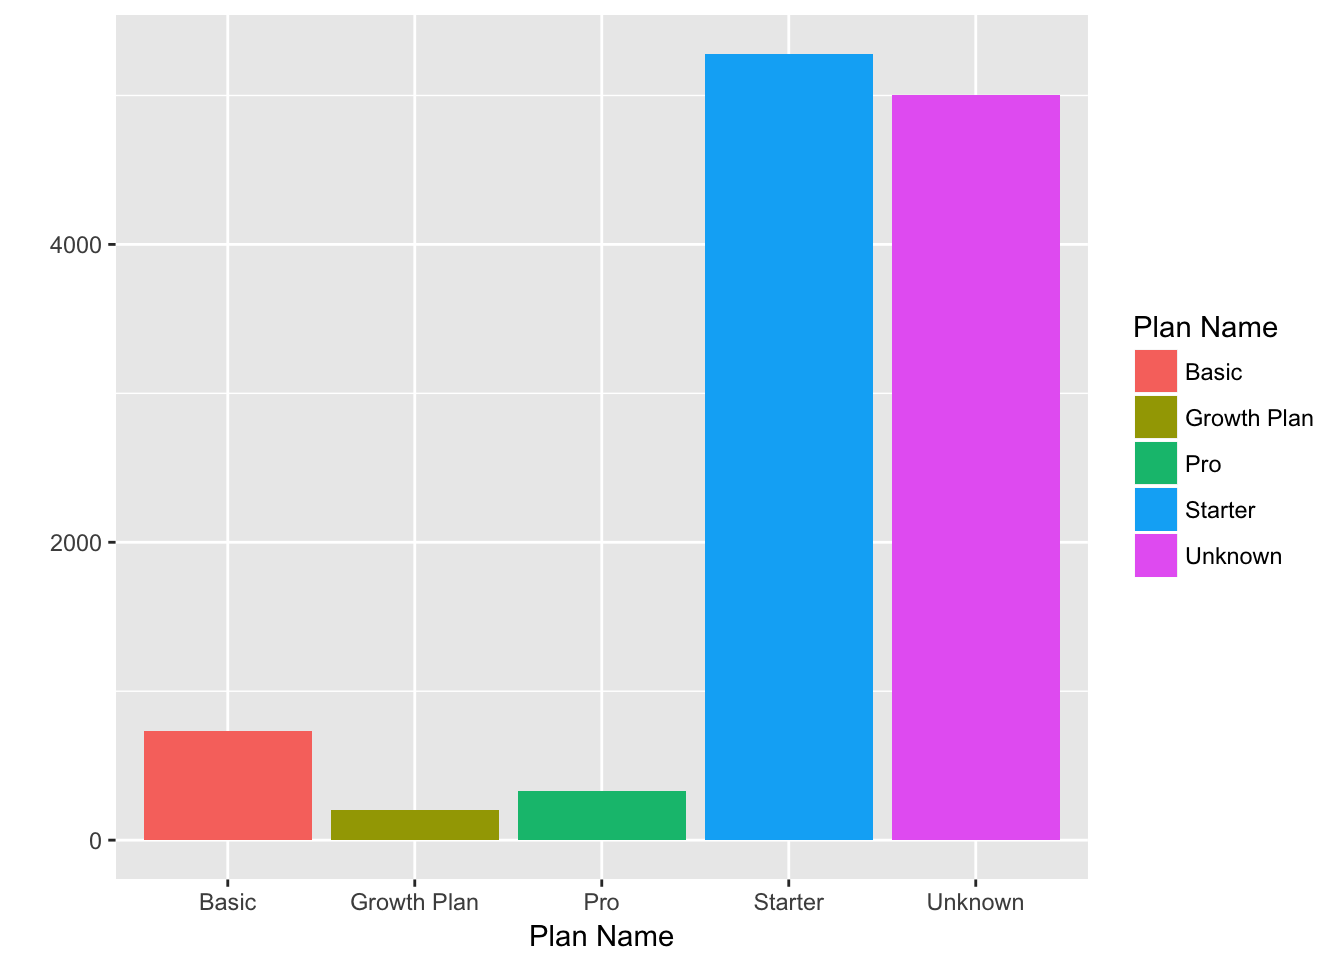
\includegraphics{capstone_project_files/figure-latex/unnamed-chunk-27-1.pdf}

\subparagraph{Paying Subscribers}\label{paying-subscribers}

Next we will focus on paying customers only. Thus, we will filter out
all the ``Unknown'' and ``Starters'' values from plan name variable.

\begin{Shaded}
\begin{Highlighting}[]
\NormalTok{wp_data_subscribed <-}\StringTok{ }\NormalTok{wp_data }\OperatorTok\StringTok{ }\KeywordTok{filter}\NormalTok{(Unsubscribed }\OperatorTok{==}\StringTok{ "FALSE"}\NormalTok{, plan_name }\OperatorTok{!=}\StringTok{ "Unknown"}\NormalTok{, plan_name }\OperatorTok{!=}\StringTok{ "Starter"}\NormalTok{)}
\end{Highlighting}
\end{Shaded}

\subparagraph{Total Amount of Leads}\label{total-amount-of-leads}

For this graph, we start with those who have acquired at least one lead,
as if we count those who haven't captured any lead, it will distort the
graph as the number is much greater than any other. This is not the best
signal as it means that there are lot of customers that are not being
able to generate any lead. Another interesting point to analyze is that
there are a lot of customers on the basic plan that have acquired more
leads than the maximum allowed under their current plan (500 leads),
which means that they upgraded their account to run a campaign and then
went back to basic plan.

\begin{Shaded}
\begin{Highlighting}[]
\KeywordTok{ggplot}\NormalTok{(wp_data_subscribed, }\KeywordTok{aes}\NormalTok{(total_leads, }\DataTypeTok{fill =}\NormalTok{ plan_name)) }\OperatorTok{+}
\StringTok{  }\KeywordTok{geom_histogram}\NormalTok{(}\DataTypeTok{breaks =} \KeywordTok{seq}\NormalTok{(}\DecValTok{1}\NormalTok{,}\DecValTok{20000}\NormalTok{, }\DataTypeTok{by =} \DecValTok{100}\NormalTok{))  }\OperatorTok{+}
\StringTok{  }\KeywordTok{labs}\NormalTok{(}\DataTypeTok{x =} \StringTok{"Total Leads"}\NormalTok{, }\DataTypeTok{y =} \StringTok{"Count"}\NormalTok{) }\OperatorTok{+}
\StringTok{  }\KeywordTok{scale_fill_discrete}\NormalTok{(}\DataTypeTok{name =} \StringTok{"Plan Name"}\NormalTok{) }
\end{Highlighting}
\end{Shaded}

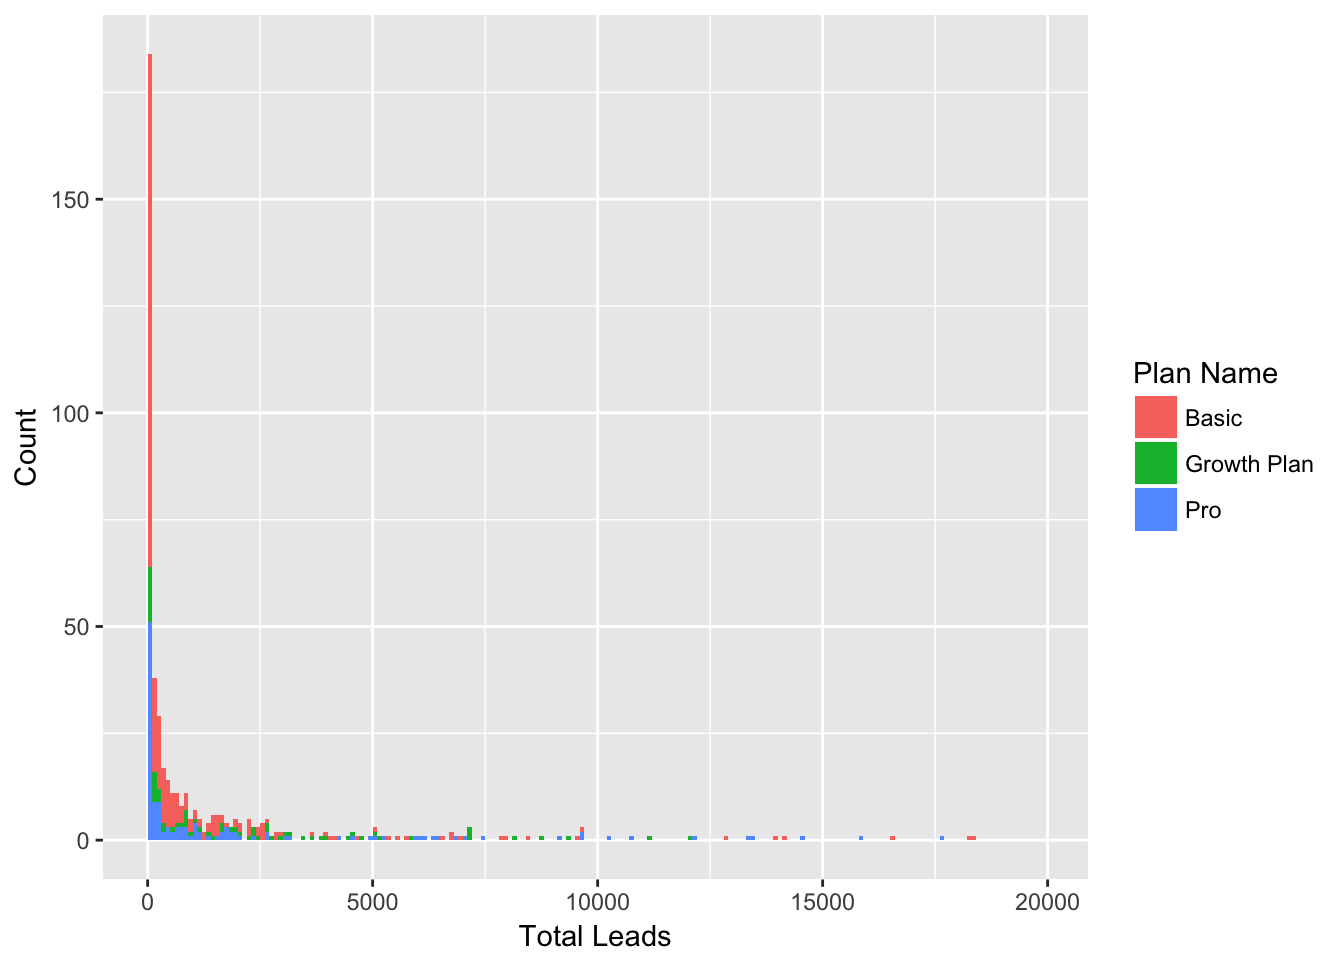
\includegraphics{capstone_project_files/figure-latex/unnamed-chunk-29-1.pdf}

\subparagraph{Total Amount of Live
Tools}\label{total-amount-of-live-tools}

For this graph, we start with those who have created at least 1 tool,
because if we count those who haven't created anything, it will distort
the graph as the number of zero live tool is much greater than any
other. Another interesting point to analyze is that most of those who
have more than 25 live tools are on the Pro and Growth plan.

\begin{Shaded}
\begin{Highlighting}[]
\KeywordTok{ggplot}\NormalTok{(wp_data_subscribed, }\KeywordTok{aes}\NormalTok{(total_live_tools, }\DataTypeTok{fill =}\NormalTok{ plan_name)) }\OperatorTok{+}
\StringTok{  }\KeywordTok{geom_histogram}\NormalTok{(}\DataTypeTok{breaks =} \KeywordTok{seq}\NormalTok{(}\DecValTok{1}\NormalTok{,}\DecValTok{150}\NormalTok{, }\DataTypeTok{by =} \DecValTok{5}\NormalTok{)) }\OperatorTok{+}
\StringTok{  }\KeywordTok{labs}\NormalTok{(}\DataTypeTok{x =} \StringTok{"Total Live Tools"}\NormalTok{, }\DataTypeTok{y =} \StringTok{"Count"}\NormalTok{) }\OperatorTok{+}
\StringTok{  }\KeywordTok{scale_fill_discrete}\NormalTok{(}\DataTypeTok{name =} \StringTok{"Plan Name"}\NormalTok{)  }
\end{Highlighting}
\end{Shaded}

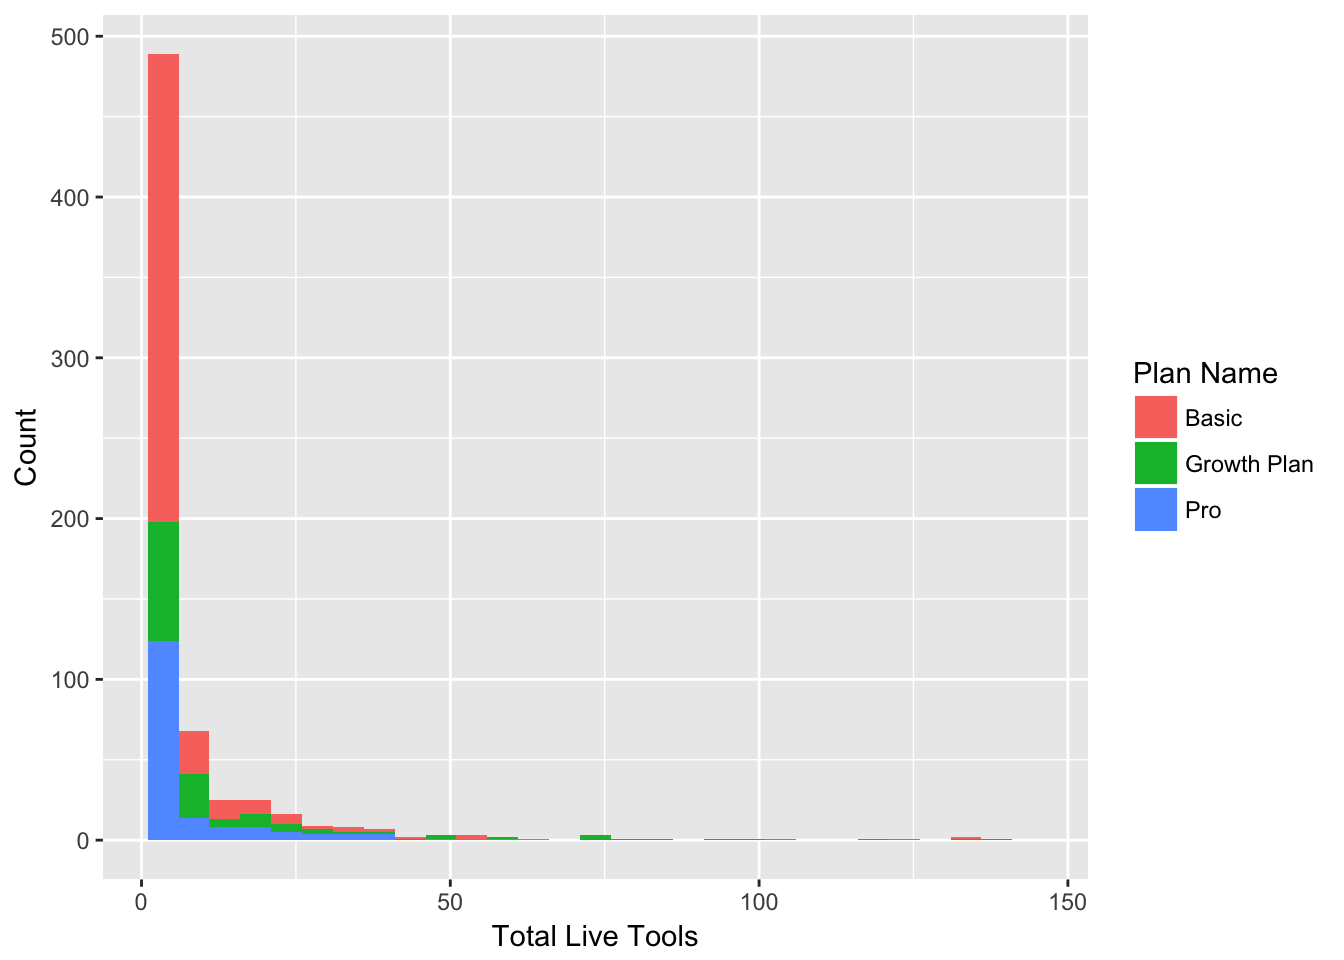
\includegraphics{capstone_project_files/figure-latex/unnamed-chunk-30-1.pdf}

\subparagraph{Sales}\label{sales}

The graph shows that most of the subscriptions are not coming through
sales agents, but through other means. The sales team is fairly
expensive with a lot of personnel. Thus, Wishpond could reduce expenses
by decreasing the sales team and increase revenue by focusing on the
different avenues that are bringing more customers.

\begin{Shaded}
\begin{Highlighting}[]
\KeywordTok{ggplot}\NormalTok{(wp_data_subscribed, }\KeywordTok{aes}\NormalTok{(}\KeywordTok{factor}\NormalTok{(wp_data_subscribed}\OperatorTok{$}\NormalTok{plan_name))) }\OperatorTok{+}
\StringTok{  }\KeywordTok{geom_bar}\NormalTok{(}\DataTypeTok{stat =} \StringTok{"count"}\NormalTok{, }\KeywordTok{aes}\NormalTok{(}\DataTypeTok{fill =} \KeywordTok{factor}\NormalTok{(wp_data_subscribed}\OperatorTok{$}\NormalTok{plan_name))) }\OperatorTok{+}
\StringTok{  }\KeywordTok{facet_grid}\NormalTok{(. }\OperatorTok{~}\StringTok{ }\KeywordTok{factor}\NormalTok{(wp_data_subscribed}\OperatorTok{$}\NormalTok{sales)) }\OperatorTok{+}
\StringTok{  }\KeywordTok{xlab}\NormalTok{(}\StringTok{"Plan Name"}\NormalTok{) }\OperatorTok{+}
\StringTok{  }\KeywordTok{scale_fill_discrete}\NormalTok{(}\DataTypeTok{name =} \StringTok{"Plan Name"}\NormalTok{)     }
\end{Highlighting}
\end{Shaded}

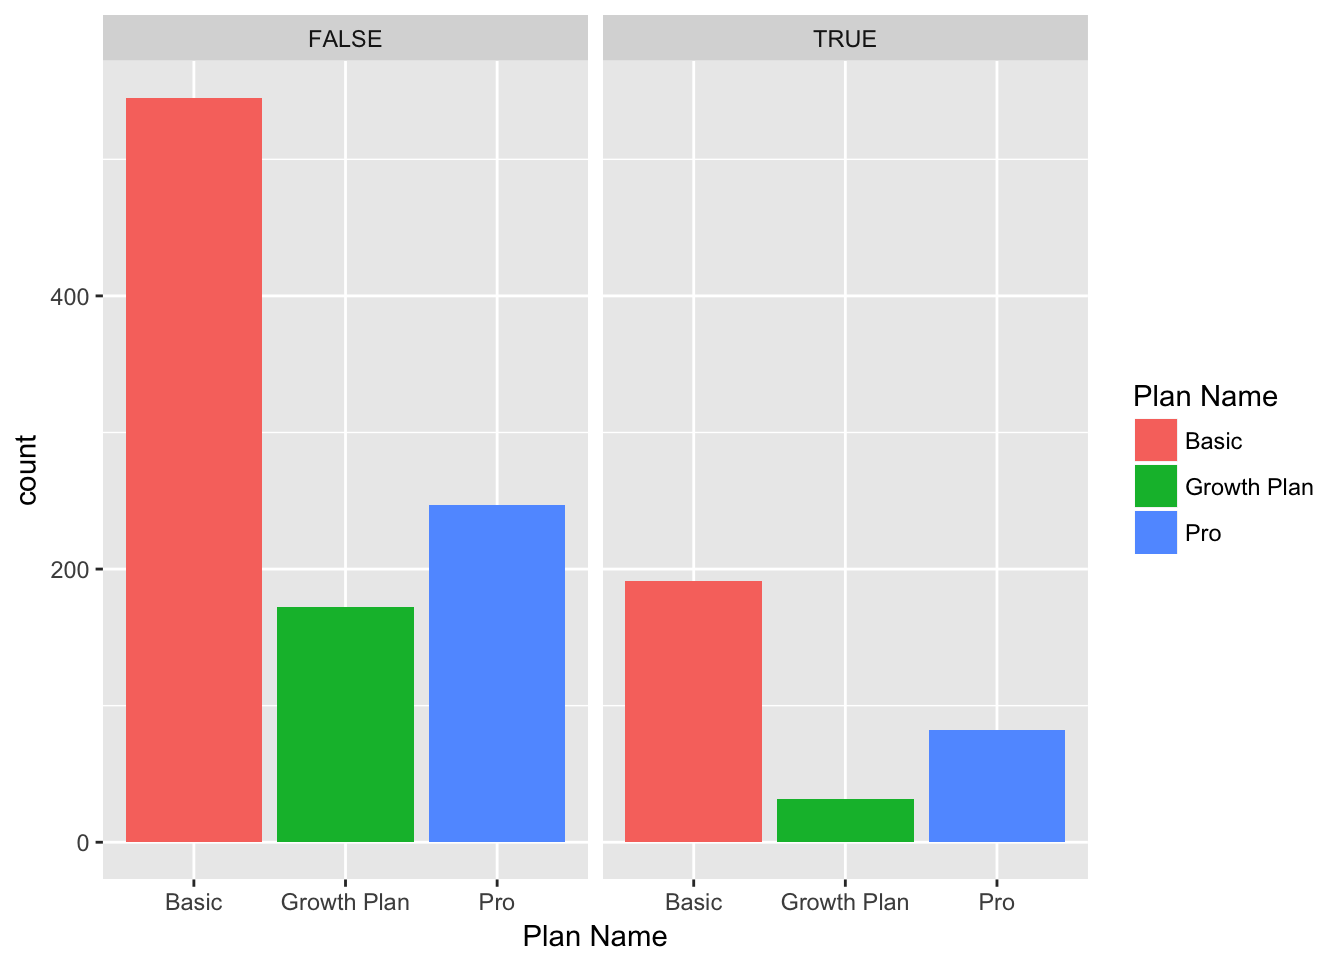
\includegraphics{capstone_project_files/figure-latex/unnamed-chunk-31-1.pdf}

\subparagraph{Affiliated}\label{affiliated}

While affiliated links have not generated as many sales as sales agents,
the number are not too far off. Also, the amount of money spent on an
affiliated link is much less than a sales agent salary. Pushing the
affiliated program could be a good alternative to bring more customers
to Wishpond at a lower cost.

\begin{Shaded}
\begin{Highlighting}[]
\KeywordTok{ggplot}\NormalTok{(wp_data_subscribed, }\KeywordTok{aes}\NormalTok{(}\KeywordTok{factor}\NormalTok{(wp_data_subscribed}\OperatorTok{$}\NormalTok{plan_name))) }\OperatorTok{+}
\StringTok{  }\KeywordTok{geom_bar}\NormalTok{(}\DataTypeTok{stat =} \StringTok{"count"}\NormalTok{, }\KeywordTok{aes}\NormalTok{(}\DataTypeTok{fill =} \KeywordTok{factor}\NormalTok{(wp_data_subscribed}\OperatorTok{$}\NormalTok{plan_name))) }\OperatorTok{+}
\StringTok{  }\KeywordTok{facet_grid}\NormalTok{(. }\OperatorTok{~}\StringTok{ }\KeywordTok{factor}\NormalTok{(wp_data_subscribed}\OperatorTok{$}\NormalTok{affiliated)) }\OperatorTok{+}
\StringTok{  }\KeywordTok{xlab}\NormalTok{(}\StringTok{"Plan Name"}\NormalTok{) }\OperatorTok{+}
\StringTok{  }\KeywordTok{ylab}\NormalTok{(}\StringTok{""}\NormalTok{) }\OperatorTok{+}
\StringTok{  }\KeywordTok{scale_fill_discrete}\NormalTok{(}\DataTypeTok{name =} \StringTok{"Plan Name"}\NormalTok{)     }
\end{Highlighting}
\end{Shaded}

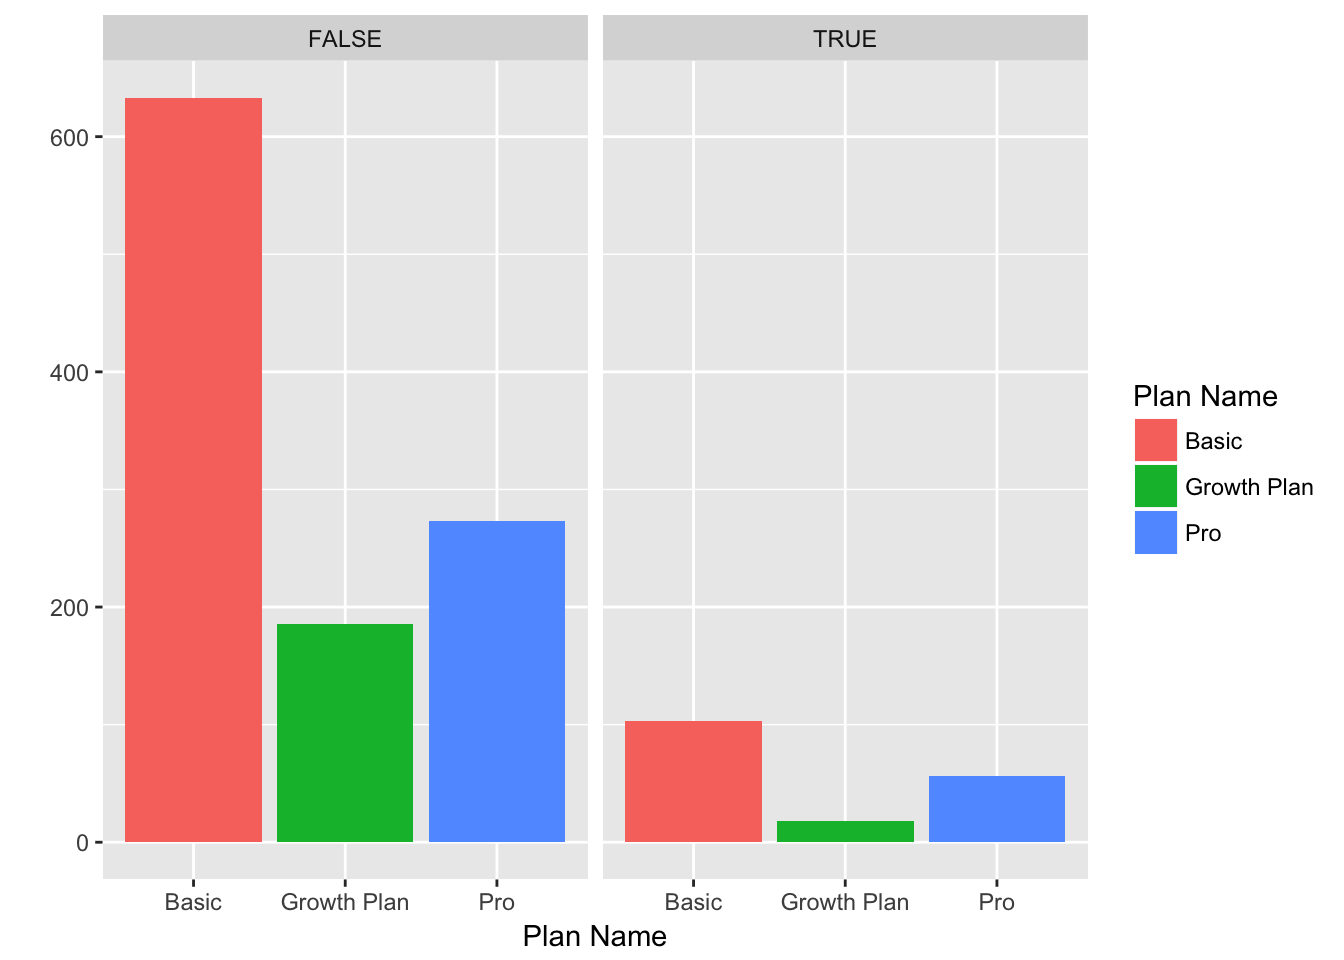
\includegraphics{capstone_project_files/figure-latex/unnamed-chunk-32-1.pdf}

\subparagraph{Have Read Wishpond Blog}\label{have-read-wishpond-blog}

The graph below shows us that those who have read the blog are
generating more leads than those who have not read the blog. Thus,
showing us that the blog might help customers to capture leads.

\begin{Shaded}
\begin{Highlighting}[]
\KeywordTok{ggplot}\NormalTok{(wp_data_subscribed, }\KeywordTok{aes}\NormalTok{(total_leads, }\DataTypeTok{fill =}\NormalTok{ plan_name)) }\OperatorTok{+}
\StringTok{  }\KeywordTok{geom_histogram}\NormalTok{(}\DataTypeTok{breaks =} \KeywordTok{seq}\NormalTok{(}\DecValTok{1}\NormalTok{,}\DecValTok{20000}\NormalTok{, }\DataTypeTok{by =} \DecValTok{100}\NormalTok{))  }\OperatorTok{+}
\StringTok{  }\KeywordTok{facet_grid}\NormalTok{(. }\OperatorTok{~}\StringTok{ }\KeywordTok{factor}\NormalTok{(wp_data_subscribed}\OperatorTok{$}\NormalTok{read_blog)) }\OperatorTok{+}
\StringTok{  }\KeywordTok{labs}\NormalTok{(}\DataTypeTok{title =} \StringTok{"Have Read The Blog?"}\NormalTok{, }\DataTypeTok{x =} \StringTok{"Total Leads"}\NormalTok{, }\DataTypeTok{y =} \StringTok{"Count"}\NormalTok{) }\OperatorTok{+}
\StringTok{  }\KeywordTok{scale_fill_discrete}\NormalTok{(}\DataTypeTok{name =} \StringTok{"Plan Name"}\NormalTok{)}
\end{Highlighting}
\end{Shaded}

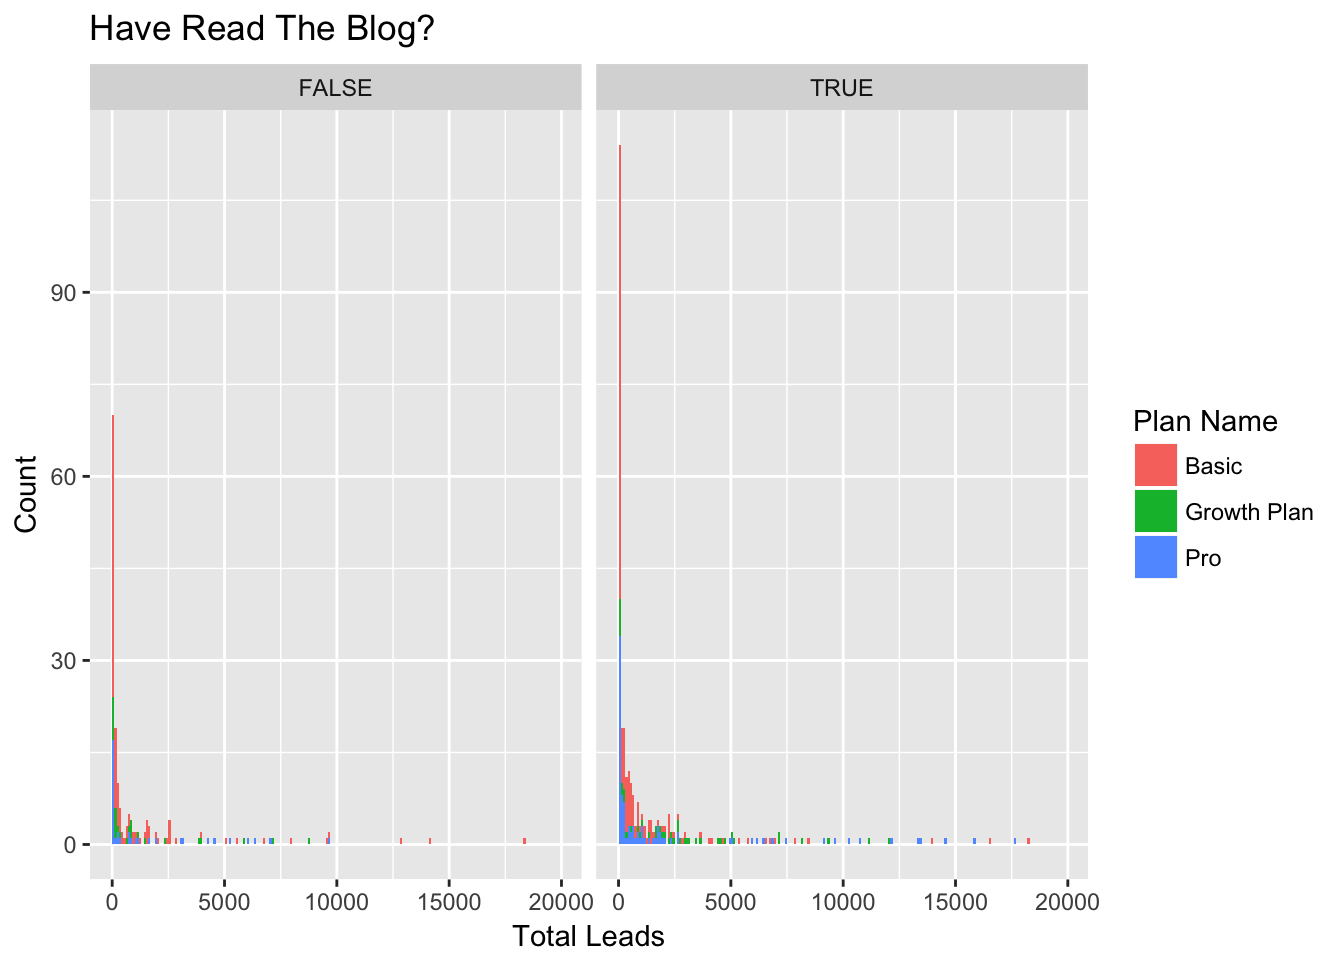
\includegraphics{capstone_project_files/figure-latex/unnamed-chunk-33-1.pdf}

\subparagraph{Have Read Wishpond Blog and Total Amount of
Leads}\label{have-read-wishpond-blog-and-total-amount-of-leads}

The graph below shows us that those who have read the blog create more
tools than those who have not. Thus, showing that the blog might
influence on supporting customer to get started with Wishpond and create
different tools on the platform.

\begin{Shaded}
\begin{Highlighting}[]
\KeywordTok{ggplot}\NormalTok{(wp_data_subscribed, }\KeywordTok{aes}\NormalTok{(total_live_tools, }\DataTypeTok{fill =}\NormalTok{ plan_name)) }\OperatorTok{+}
\StringTok{  }\KeywordTok{geom_histogram}\NormalTok{(}\DataTypeTok{breaks =} \KeywordTok{seq}\NormalTok{(}\DecValTok{1}\NormalTok{,}\DecValTok{150}\NormalTok{, }\DataTypeTok{by =} \DecValTok{5}\NormalTok{)) }\OperatorTok{+}
\StringTok{  }\KeywordTok{facet_grid}\NormalTok{(. }\OperatorTok{~}\StringTok{ }\KeywordTok{factor}\NormalTok{(wp_data_subscribed}\OperatorTok{$}\NormalTok{read_blog)) }\OperatorTok{+}
\StringTok{  }\KeywordTok{labs}\NormalTok{(}\DataTypeTok{title =} \StringTok{"Have Read The Blog?"}\NormalTok{, }\DataTypeTok{x =} \StringTok{"Total Live Tools"}\NormalTok{, }\DataTypeTok{y =} \StringTok{"Count"}\NormalTok{) }\OperatorTok{+}
\StringTok{  }\KeywordTok{scale_fill_discrete}\NormalTok{(}\DataTypeTok{name =} \StringTok{"Plan Name"}\NormalTok{)  }
\end{Highlighting}
\end{Shaded}

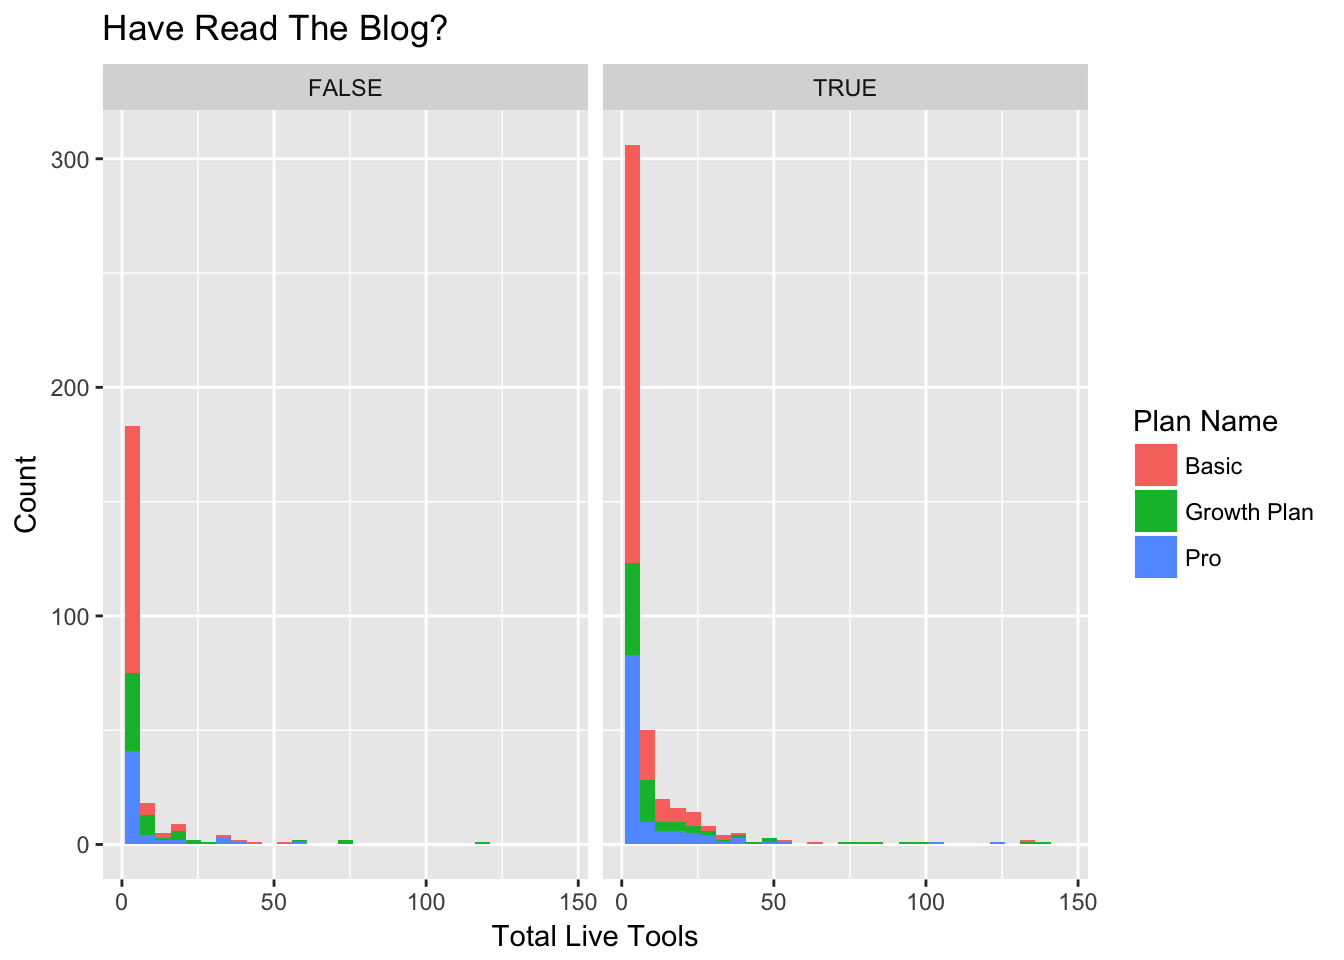
\includegraphics{capstone_project_files/figure-latex/unnamed-chunk-34-1.pdf}

\subparagraph{Have Read Wishpond Blog and Total Amount of
Leads}\label{have-read-wishpond-blog-and-total-amount-of-leads-1}

Similar to the amount of leads, we want to see how the blog is
influencing customers on creating different tools at Wishpond. The
interesting factor on this graph is that most of the customers that have
read the blog are not using Wishpond tools as much as those who have not
read it. Therefore, Wishpond should allocate some space to talk about
the importance of using workflows, pop-up and other tools, in order to
get customers to use more of Wishpond tools.

\begin{Shaded}
\begin{Highlighting}[]
\KeywordTok{ggplot}\NormalTok{(wp_data_subscribed, }\KeywordTok{aes}\NormalTok{(}\KeywordTok{factor}\NormalTok{(wp_data_subscribed}\OperatorTok{$}\NormalTok{total_live_tools))) }\OperatorTok{+}
\StringTok{  }\KeywordTok{geom_bar}\NormalTok{(}\DataTypeTok{stat =} \StringTok{"count"}\NormalTok{, }\KeywordTok{aes}\NormalTok{(}\DataTypeTok{fill =} \KeywordTok{factor}\NormalTok{(wp_data_subscribed}\OperatorTok{$}\NormalTok{total_live_tools))) }\OperatorTok{+}
\StringTok{  }\KeywordTok{facet_grid}\NormalTok{(. }\OperatorTok{~}\StringTok{ }\KeywordTok{factor}\NormalTok{(wp_data_subscribed}\OperatorTok{$}\NormalTok{read_blog)) }\OperatorTok{+}
\StringTok{  }\KeywordTok{xlab}\NormalTok{(}\StringTok{"Total Live Tools"}\NormalTok{) }\OperatorTok{+}
\StringTok{  }\KeywordTok{ylab}\NormalTok{(}\StringTok{""}\NormalTok{) }\OperatorTok{+}
\StringTok{  }\KeywordTok{scale_fill_discrete}\NormalTok{(}\DataTypeTok{name =} \StringTok{"Total Live Tools"}\NormalTok{)}
\end{Highlighting}
\end{Shaded}

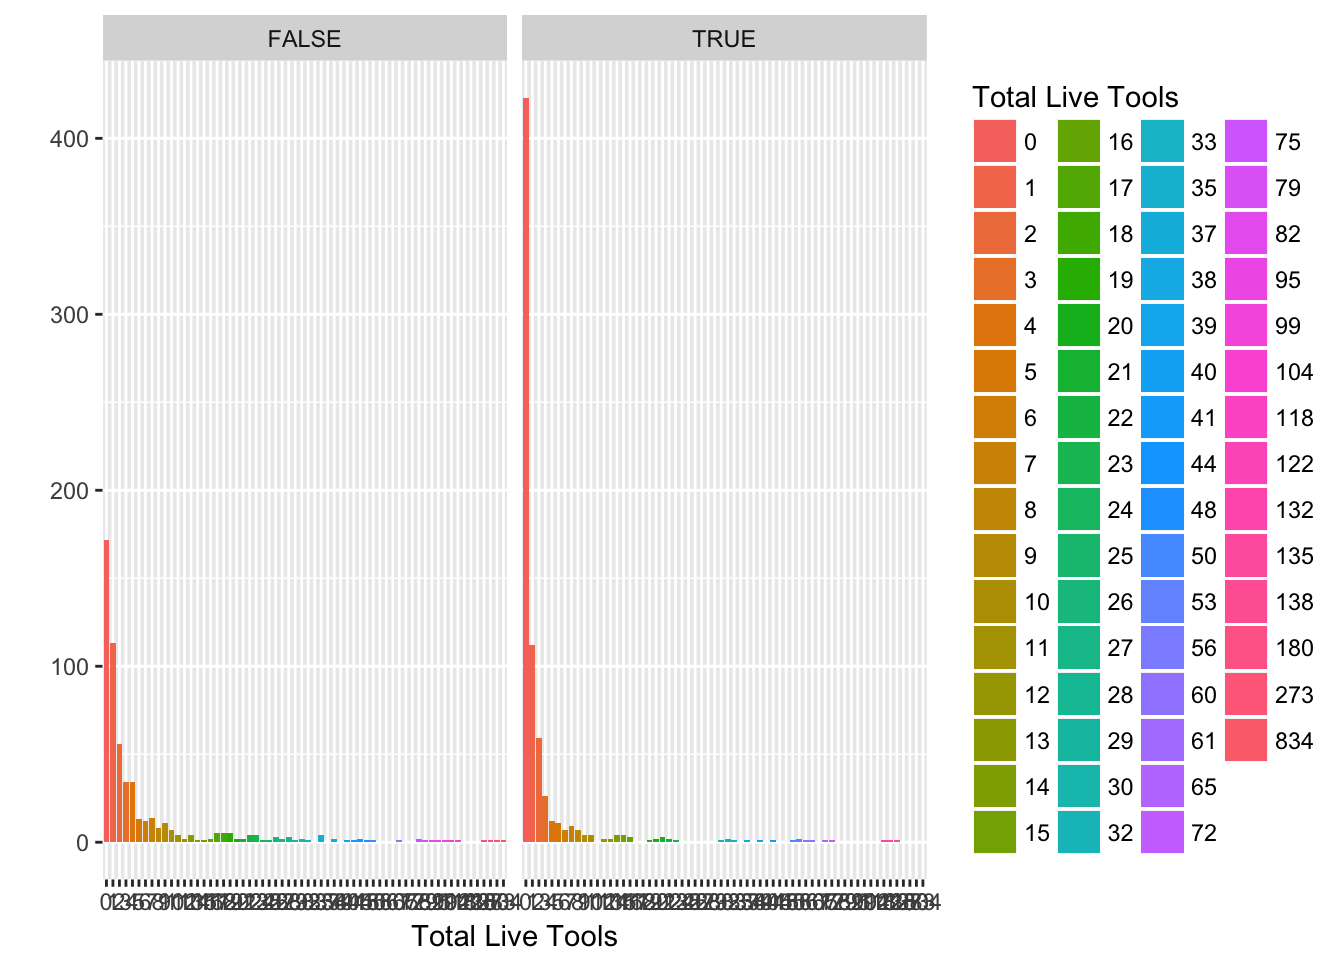
\includegraphics{capstone_project_files/figure-latex/unnamed-chunk-35-1.pdf}

\subparagraph{Business Industry At Each
Plan}\label{business-industry-at-each-plan}

From the graph below we can see that e-commerce is the leading business
industry on Wishpond, while agency has a good share of customers. By
analysing the graph for the starter plan, we can understand where most
of the opportunity to turn customers to paid customers are, e-commerce
and agency. At the Growth plan, the most expensive plan, e-commerce is
by far the most predominant business industry. Thus, it allows us to see
where Wishpond should start focusing in order to bring more customers.

Starter Plan \& Business Industry

\begin{Shaded}
\begin{Highlighting}[]
\NormalTok{wp_data_starter <-}\StringTok{ }\NormalTok{wp_data }\OperatorTok\StringTok{ }\KeywordTok{filter}\NormalTok{(plan_name }\OperatorTok{==}\StringTok{ "Starter"}\NormalTok{, Unsubscribed }\OperatorTok{==}\StringTok{ "FALSE"}\NormalTok{, business_industry }\OperatorTok{!=}\StringTok{ "Other"}\NormalTok{, business_industry }\OperatorTok{!=}\StringTok{ "Unknown"}\NormalTok{)}
\KeywordTok{ggplot}\NormalTok{(wp_data_starter, }\KeywordTok{aes}\NormalTok{(}\KeywordTok{factor}\NormalTok{(wp_data_starter}\OperatorTok{$}\NormalTok{business_industry))) }\OperatorTok{+}
\StringTok{  }\KeywordTok{geom_bar}\NormalTok{(}\DataTypeTok{stat =} \StringTok{"count"}\NormalTok{, }\KeywordTok{aes}\NormalTok{(}\DataTypeTok{fill =} \KeywordTok{factor}\NormalTok{(wp_data_starter}\OperatorTok{$}\NormalTok{business_industry))) }\OperatorTok{+}
\StringTok{  }\KeywordTok{facet_grid}\NormalTok{(. }\OperatorTok{~}\StringTok{ }\KeywordTok{factor}\NormalTok{(wp_data_starter}\OperatorTok{$}\NormalTok{plan_name)) }\OperatorTok{+}
\StringTok{  }\KeywordTok{xlab}\NormalTok{(}\StringTok{"business industry"}\NormalTok{) }\OperatorTok{+}
\StringTok{  }\KeywordTok{ylab}\NormalTok{(}\StringTok{""}\NormalTok{) }\OperatorTok{+}
\StringTok{  }\KeywordTok{scale_fill_discrete}\NormalTok{(}\DataTypeTok{name =} \StringTok{"business industry"}\NormalTok{)     }
\end{Highlighting}
\end{Shaded}

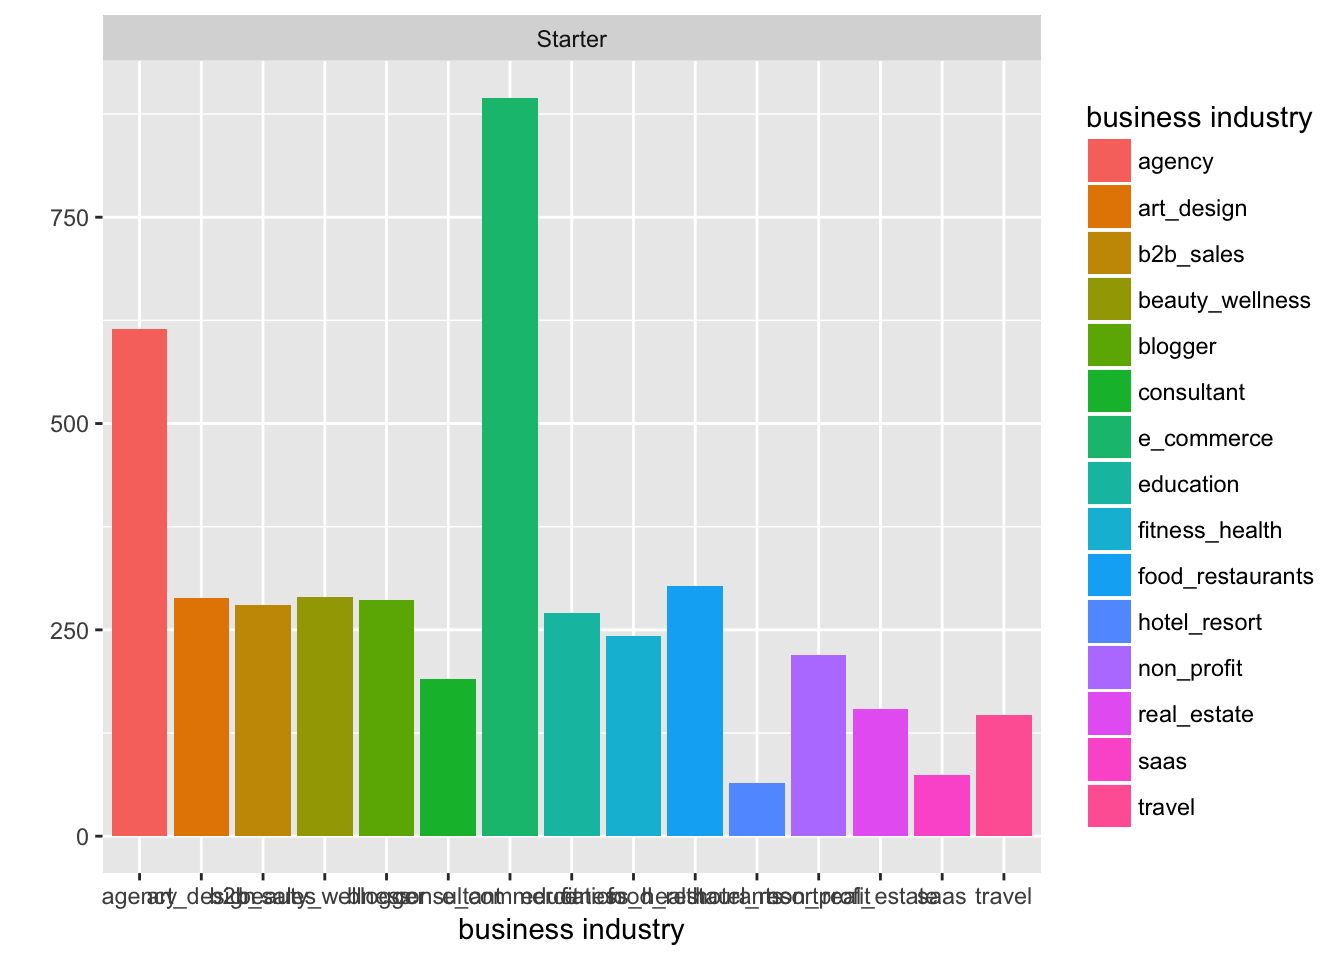
\includegraphics{capstone_project_files/figure-latex/unnamed-chunk-36-1.pdf}

Basic Plan \& Business Industry

\begin{Shaded}
\begin{Highlighting}[]
\NormalTok{wp_data_basic <-}\StringTok{ }\NormalTok{wp_data }\OperatorTok\StringTok{ }\KeywordTok{filter}\NormalTok{(plan_name }\OperatorTok{==}\StringTok{ "Basic"}\NormalTok{, Unsubscribed }\OperatorTok{==}\StringTok{ "FALSE"}\NormalTok{, business_industry }\OperatorTok{!=}\StringTok{ "Other"}\NormalTok{, business_industry }\OperatorTok{!=}\StringTok{ "Unknown"}\NormalTok{)}
\KeywordTok{ggplot}\NormalTok{(wp_data_basic, }\KeywordTok{aes}\NormalTok{(}\KeywordTok{factor}\NormalTok{(wp_data_basic}\OperatorTok{$}\NormalTok{business_industry))) }\OperatorTok{+}
\StringTok{  }\KeywordTok{geom_bar}\NormalTok{(}\DataTypeTok{stat =} \StringTok{"count"}\NormalTok{, }\KeywordTok{aes}\NormalTok{(}\DataTypeTok{fill =} \KeywordTok{factor}\NormalTok{(wp_data_basic}\OperatorTok{$}\NormalTok{business_industry))) }\OperatorTok{+}
\StringTok{  }\KeywordTok{facet_grid}\NormalTok{(. }\OperatorTok{~}\StringTok{ }\KeywordTok{factor}\NormalTok{(wp_data_basic}\OperatorTok{$}\NormalTok{plan_name)) }\OperatorTok{+}
\StringTok{  }\KeywordTok{xlab}\NormalTok{(}\StringTok{"business industry"}\NormalTok{) }\OperatorTok{+}
\StringTok{  }\KeywordTok{ylab}\NormalTok{(}\StringTok{""}\NormalTok{) }\OperatorTok{+}
\StringTok{  }\KeywordTok{scale_fill_discrete}\NormalTok{(}\DataTypeTok{name =} \StringTok{"business industry"}\NormalTok{)    }
\end{Highlighting}
\end{Shaded}

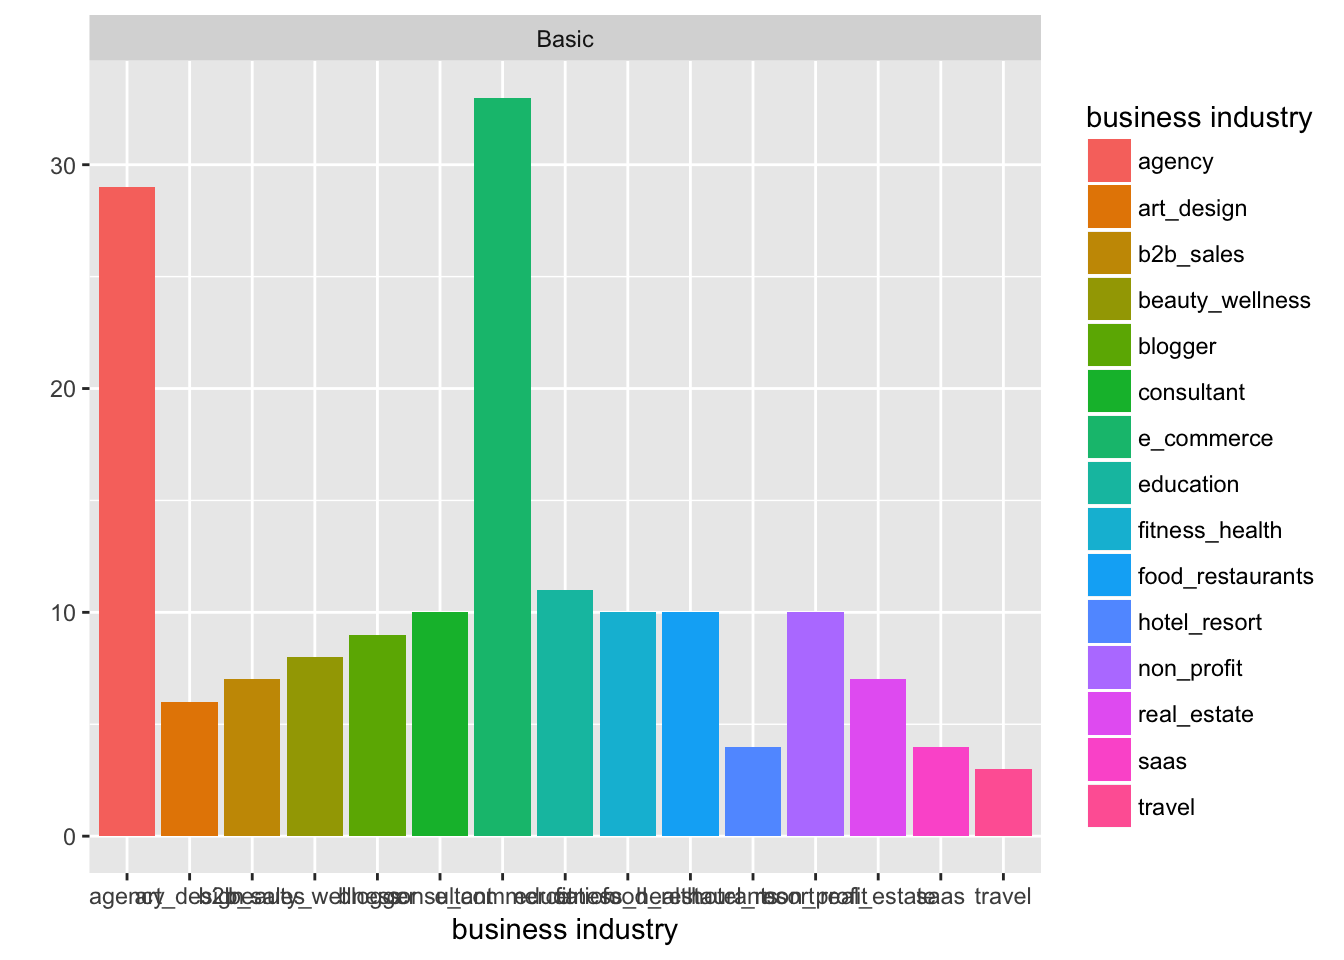
\includegraphics{capstone_project_files/figure-latex/unnamed-chunk-37-1.pdf}

Pro Plan \& Business Industry \textbar{} Second Most Expensive Plan
\textbar{} E-Commerce by far the most relevant one. Art-design and
fitness health industry coming in second

\begin{Shaded}
\begin{Highlighting}[]
\NormalTok{wp_data_pro <-}\StringTok{ }\NormalTok{wp_data }\OperatorTok\StringTok{ }\KeywordTok{filter}\NormalTok{(plan_name }\OperatorTok{==}\StringTok{ "Pro"}\NormalTok{, Unsubscribed }\OperatorTok{==}\StringTok{ "FALSE"}\NormalTok{, business_industry }\OperatorTok{!=}\StringTok{ "Other"}\NormalTok{, business_industry }\OperatorTok{!=}\StringTok{ "Unknown"}\NormalTok{)}
\KeywordTok{ggplot}\NormalTok{(wp_data_pro, }\KeywordTok{aes}\NormalTok{(}\KeywordTok{factor}\NormalTok{(wp_data_pro}\OperatorTok{$}\NormalTok{business_industry))) }\OperatorTok{+}
\StringTok{  }\KeywordTok{geom_bar}\NormalTok{(}\DataTypeTok{stat =} \StringTok{"count"}\NormalTok{, }\KeywordTok{aes}\NormalTok{(}\DataTypeTok{fill =} \KeywordTok{factor}\NormalTok{(wp_data_pro}\OperatorTok{$}\NormalTok{business_industry))) }\OperatorTok{+}
\StringTok{  }\KeywordTok{facet_grid}\NormalTok{(. }\OperatorTok{~}\StringTok{ }\KeywordTok{factor}\NormalTok{(wp_data_pro}\OperatorTok{$}\NormalTok{plan_name)) }\OperatorTok{+}
\StringTok{  }\KeywordTok{xlab}\NormalTok{(}\StringTok{"business industry"}\NormalTok{) }\OperatorTok{+}
\StringTok{  }\KeywordTok{ylab}\NormalTok{(}\StringTok{""}\NormalTok{) }\OperatorTok{+}
\StringTok{  }\KeywordTok{scale_fill_discrete}\NormalTok{(}\DataTypeTok{name =} \StringTok{"business industry"}\NormalTok{)     }
\end{Highlighting}
\end{Shaded}

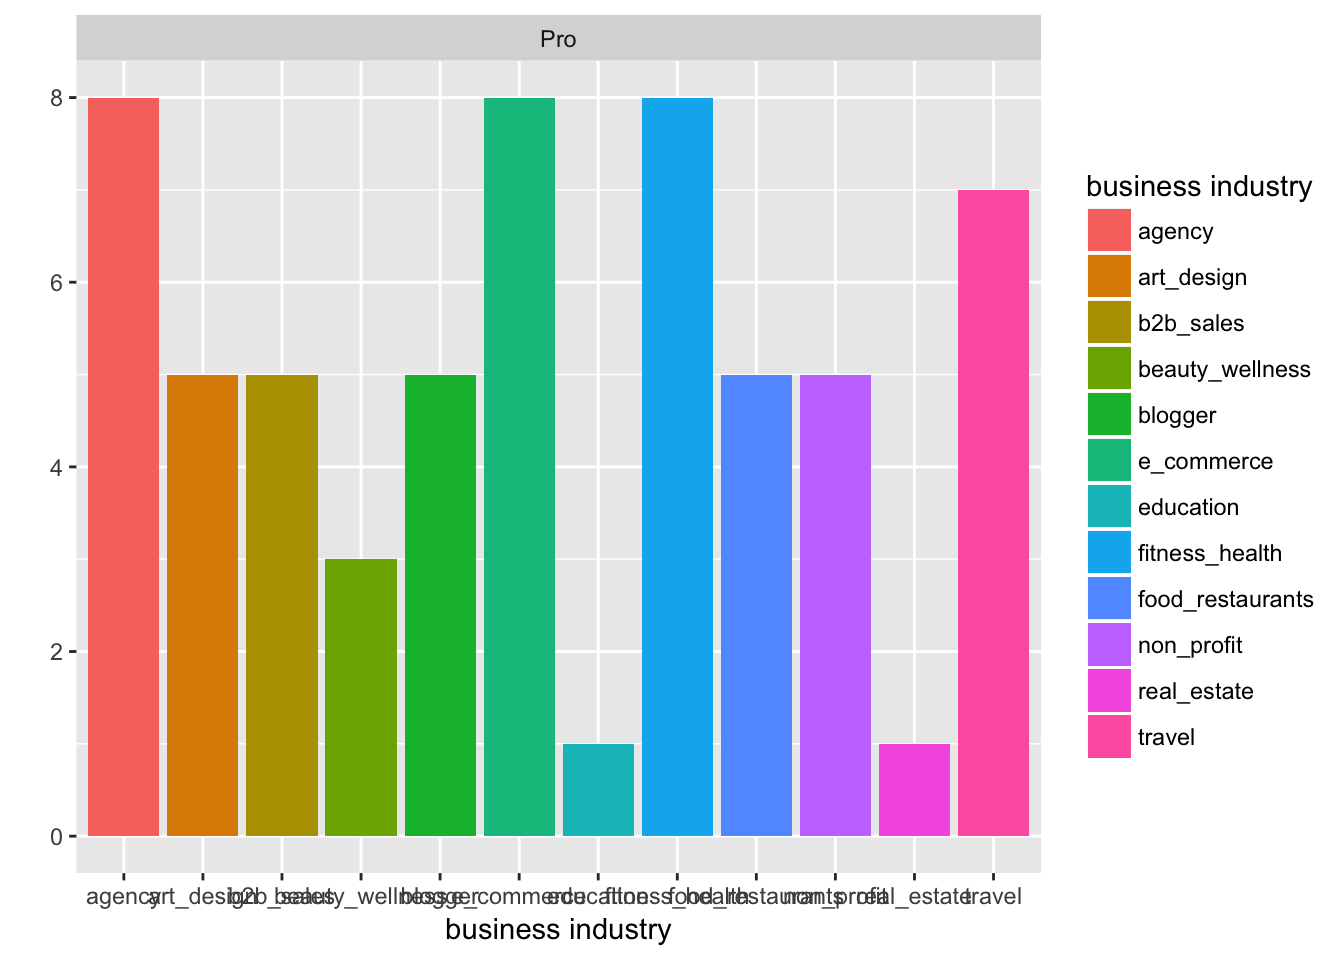
\includegraphics{capstone_project_files/figure-latex/unnamed-chunk-38-1.pdf}

Growth Plan \& Business \textbar{} Most Expensive Plan \textbar{}
E-Commerce by far again bringing the most customers to Growth plan.

\begin{Shaded}
\begin{Highlighting}[]
\NormalTok{wp_data_growth <-}\StringTok{ }\NormalTok{wp_data }\OperatorTok\StringTok{ }\KeywordTok{filter}\NormalTok{(plan_name }\OperatorTok{==}\StringTok{ "Growth Plan"}\NormalTok{, Unsubscribed }\OperatorTok{==}\StringTok{ "FALSE"}\NormalTok{, business_industry }\OperatorTok{!=}\StringTok{ "Other"}\NormalTok{, business_industry }\OperatorTok{!=}\StringTok{ "Unknown"}\NormalTok{)}
\KeywordTok{ggplot}\NormalTok{(wp_data_growth, }\KeywordTok{aes}\NormalTok{(}\KeywordTok{factor}\NormalTok{(wp_data_growth}\OperatorTok{$}\NormalTok{business_industry))) }\OperatorTok{+}
\StringTok{  }\KeywordTok{geom_bar}\NormalTok{(}\DataTypeTok{stat =} \StringTok{"count"}\NormalTok{, }\KeywordTok{aes}\NormalTok{(}\DataTypeTok{fill =} \KeywordTok{factor}\NormalTok{(wp_data_growth}\OperatorTok{$}\NormalTok{business_industry))) }\OperatorTok{+}
\StringTok{  }\KeywordTok{facet_grid}\NormalTok{(. }\OperatorTok{~}\StringTok{ }\KeywordTok{factor}\NormalTok{(wp_data_growth}\OperatorTok{$}\NormalTok{plan_name)) }\OperatorTok{+}
\StringTok{  }\KeywordTok{xlab}\NormalTok{(}\StringTok{"business industry"}\NormalTok{) }\OperatorTok{+}
\StringTok{  }\KeywordTok{ylab}\NormalTok{(}\StringTok{""}\NormalTok{) }\OperatorTok{+}
\StringTok{  }\KeywordTok{scale_fill_discrete}\NormalTok{(}\DataTypeTok{name =} \StringTok{"business industry"}\NormalTok{)     }
\end{Highlighting}
\end{Shaded}

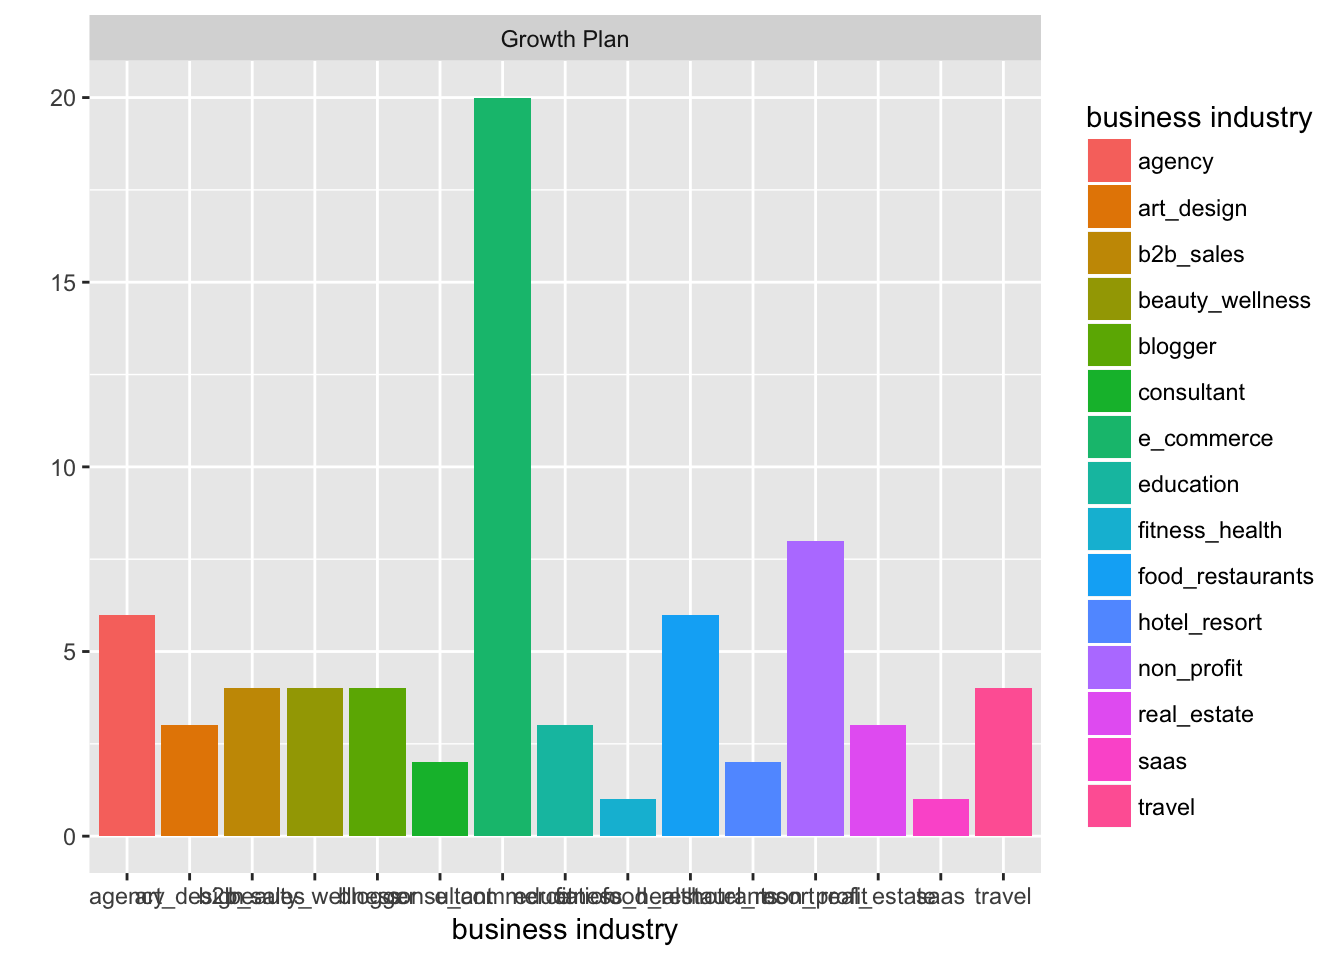
\includegraphics{capstone_project_files/figure-latex/unnamed-chunk-39-1.pdf}

\subparagraph{Business Industry and
Unsubscribed}\label{business-industry-and-unsubscribed}

The graph below shows us that e-commerce and agency are the business
industries with the most cancels, similar to the highest amount of
customers. However, by knowing that these are the greatest numbers of
cancel, we can learn what keep customers from these business industries
subscribeed at Wishpond and eventually decrease the number of cancels.

\begin{Shaded}
\begin{Highlighting}[]
\NormalTok{wp_data_unsubscribed <-}\StringTok{ }\NormalTok{wp_data }\OperatorTok\StringTok{ }\KeywordTok{filter}\NormalTok{(Unsubscribed }\OperatorTok{==}\StringTok{ "TRUE"}\NormalTok{, business_industry }\OperatorTok{!=}\StringTok{ "Other"}\NormalTok{, business_industry }\OperatorTok{!=}\StringTok{ "Unknown"}\NormalTok{)}
\KeywordTok{ggplot}\NormalTok{(wp_data_unsubscribed, }\KeywordTok{aes}\NormalTok{(}\KeywordTok{factor}\NormalTok{(wp_data_unsubscribed}\OperatorTok{$}\NormalTok{business_industry))) }\OperatorTok{+}
\StringTok{  }\KeywordTok{geom_bar}\NormalTok{(}\DataTypeTok{stat =} \StringTok{"count"}\NormalTok{, }\KeywordTok{aes}\NormalTok{(}\DataTypeTok{fill =} \KeywordTok{factor}\NormalTok{(wp_data_unsubscribed}\OperatorTok{$}\NormalTok{business_industry))) }\OperatorTok{+}
\StringTok{  }\KeywordTok{xlab}\NormalTok{(}\StringTok{"Business Industry"}\NormalTok{) }\OperatorTok{+}
\StringTok{  }\KeywordTok{ylab}\NormalTok{(}\StringTok{""}\NormalTok{) }\OperatorTok{+}
\StringTok{  }\KeywordTok{scale_fill_discrete}\NormalTok{(}\DataTypeTok{name =} \StringTok{"Business Industry"}\NormalTok{)        }
\end{Highlighting}
\end{Shaded}

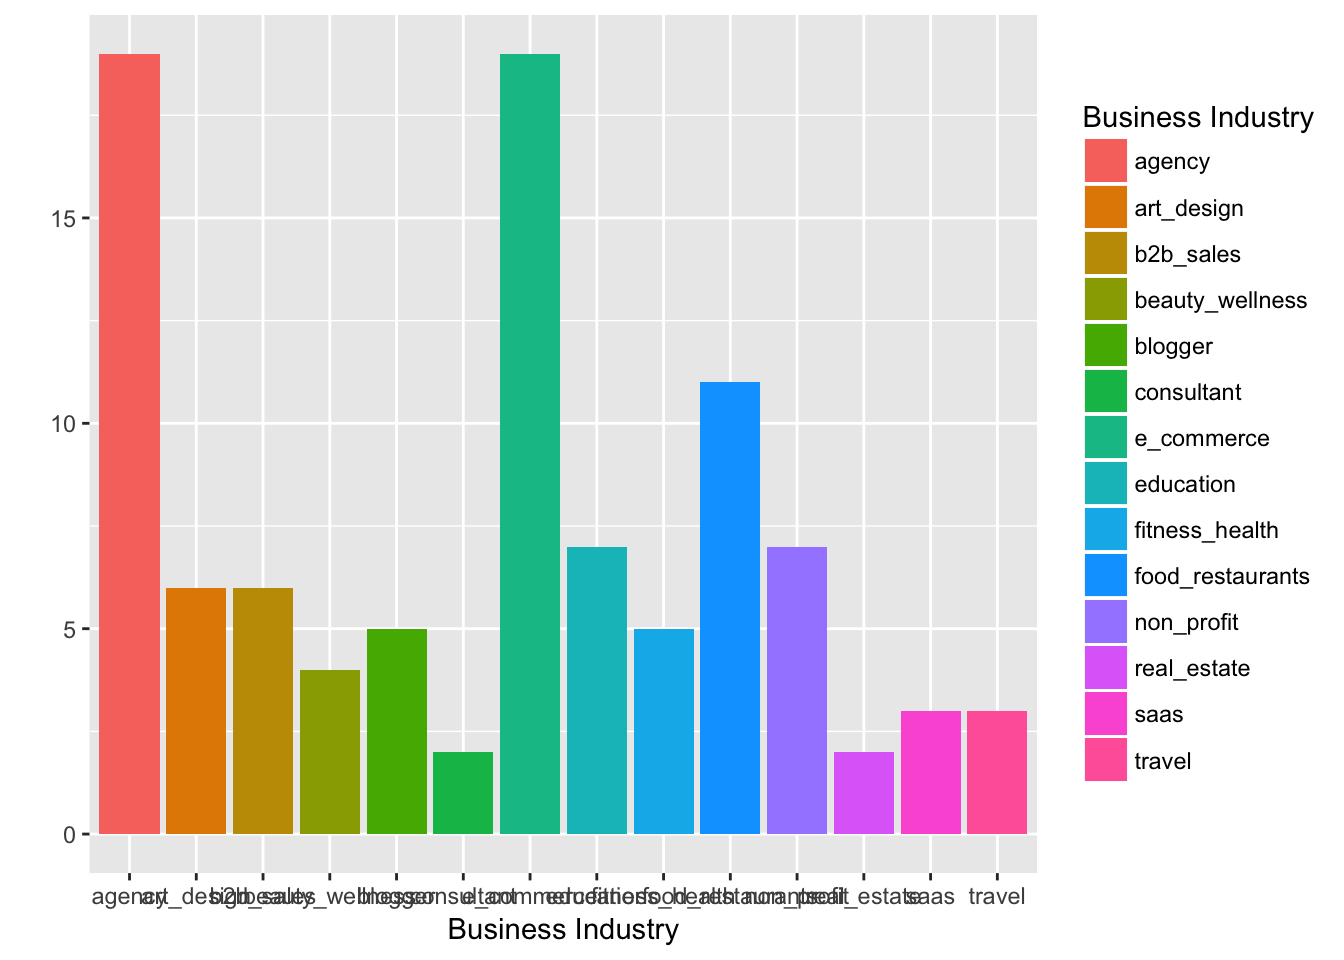
\includegraphics{capstone_project_files/figure-latex/unnamed-chunk-40-1.pdf}

\subsubsection{Machine Learning}\label{machine-learning}

\paragraph{Overview}\label{overview}

\subparagraph{This project will use machine learning to predict the risk
of a customer unsubscribing from
Wishpond.}\label{this-project-will-use-machine-learning-to-predict-the-risk-of-a-customer-unsubscribing-from-wishpond.}

\subparagraph{This is a supervised problem because we are attempting to
predict a specific dependent variable using a model based on a set of
independent
variables.}\label{this-is-a-supervised-problem-because-we-are-attempting-to-predict-a-specific-dependent-variable-using-a-model-based-on-a-set-of-independent-variables.}

\subparagraph{This is a classfication
problem}\label{this-is-a-classfication-problem}

\subparagraph{The independent variable is Unsubscribed, FALSE or
TRUE.}\label{the-independent-variable-is-unsubscribed-false-or-true.}

\subparagraph{This project used different techniques, first it used
multiple imputation to replace the missing values with plausible values
through probability. Secondly, it used Lasso Regularization to identify
the variables that may cause overfitting to our model. Lastly, it used
two different predictive models to evaluate which can perform better,
logisitic regression and random forest
regression.}\label{this-project-used-different-techniques-first-it-used-multiple-imputation-to-replace-the-missing-values-with-plausible-values-through-probability.-secondly-it-used-lasso-regularization-to-identify-the-variables-that-may-cause-overfitting-to-our-model.-lastly-it-used-two-different-predictive-models-to-evaluate-which-can-perform-better-logisitic-regression-and-random-forest-regression.}

\subparagraph{To test the predictive models, the data will be split into
two different datasets train and
test.}\label{to-test-the-predictive-models-the-data-will-be-split-into-two-different-datasets-train-and-test.}

\subparagraph{To evaluate the predictive models the data will be
splitted into two different datasets train (holding larger data) and
test (holding a smaller amount of data), in order to provide an unbiased
evaluation of the final
model.}\label{to-evaluate-the-predictive-models-the-data-will-be-splitted-into-two-different-datasets-train-holding-larger-data-and-test-holding-a-smaller-amount-of-data-in-order-to-provide-an-unbiased-evaluation-of-the-final-model.}

\subparagraph{After comparing the two models, random forest regression
producde a better model than the logistic regression for over 1\%, with
an accuracy of
76.1\%}\label{after-comparing-the-two-models-random-forest-regression-producde-a-better-model-than-the-logistic-regression-for-over-1-with-an-accuracy-of-76.1}

\paragraph{Code}\label{code}

Because our goal is to identify who are at risk of unsubscribing, we
will filter the database to those who are paying and who have
unsubscribed from the platform

\begin{Shaded}
\begin{Highlighting}[]
\NormalTok{wp_data_ml <-}\StringTok{ }\NormalTok{wp_data}
\NormalTok{wp_data_ml <-}\StringTok{ }\NormalTok{wp_data_ml }\OperatorTok\StringTok{ }\KeywordTok{filter}\NormalTok{( plan_name }\OperatorTok{==}\StringTok{ "Basic"} \OperatorTok{|}\StringTok{ }\NormalTok{plan_name }\OperatorTok{==}\StringTok{ "Pro"} \OperatorTok{|}\StringTok{ }\NormalTok{plan_name }\OperatorTok{==}\StringTok{ "Growth"} \OperatorTok{|}\StringTok{ }\NormalTok{Unsubscribed }\OperatorTok{==}\StringTok{ "TRUE"}\NormalTok{)}
\end{Highlighting}
\end{Shaded}

The database has a lot of missing values, which are described as
``Unknown'' or as ``Other'' in the database. Therefore, we will replace
these values with NAs in order to use multiple imputation and replace
with predicted values rather than ``Unknown'' and ``Other''

\begin{Shaded}
\begin{Highlighting}[]
\NormalTok{wp_data_ml[wp_data_ml }\OperatorTok{==}\StringTok{ "Unknown"}\NormalTok{] <-}\StringTok{ }\OtherTok{NA}
\NormalTok{wp_data_ml[wp_data_ml }\OperatorTok{==}\StringTok{ "Other"}\NormalTok{] <-}\StringTok{ }\OtherTok{NA}
\end{Highlighting}
\end{Shaded}

Some support agents have really low amount of customers because they are
no longer with the company. Therefore, we will exclude those with
minimun amount of customer to be replaced with NA and later be replaced
with multiple imputation.

\begin{Shaded}
\begin{Highlighting}[]
\NormalTok{support_agent_del <-}\StringTok{ }\NormalTok{wp_data_ml }\OperatorTok\StringTok{ }\KeywordTok{group_by}\NormalTok{(support_agent) }\OperatorTok\StringTok{ }\KeywordTok{filter}\NormalTok{(}\KeywordTok{n}\NormalTok{() }\OperatorTok{<}\StringTok{ }\DecValTok{10}\NormalTok{)}
\NormalTok{support_agent_del}\OperatorTok{$}\NormalTok{support_agent <-}\StringTok{ }\OtherTok{NA}
\NormalTok{support_agent_ml <-}\StringTok{ }\NormalTok{wp_data_ml }\OperatorTok\StringTok{ }\KeywordTok{group_by}\NormalTok{(support_agent)  }\OperatorTok\StringTok{ }\KeywordTok{filter}\NormalTok{(}\KeywordTok{n}\NormalTok{() }\OperatorTok{>=}\StringTok{ }\DecValTok{10}\NormalTok{)}
\NormalTok{support_agent_ml <-}\StringTok{ }\KeywordTok{bind_rows}\NormalTok{(support_agent_del, support_agent_ml)}
\NormalTok{wp_data_ml}\OperatorTok{$}\NormalTok{support_agent <-}\StringTok{ }\NormalTok{support_agent_ml}\OperatorTok{$}\NormalTok{support_agent}
\end{Highlighting}
\end{Shaded}

When customers unsubscribe, they are automatically sent to Starter plan,
which means that Starter is not the plan they were subscribed to. Thus,
we will turn all the starters plan to NAs and then use multiple
imputation to replace it with the possible plans the were once
subscribed to.

\begin{Shaded}
\begin{Highlighting}[]
\NormalTok{wp_data_ml}\OperatorTok{$}\NormalTok{plan_name[wp_data_ml}\OperatorTok{$}\NormalTok{plan_name }\OperatorTok{==}\StringTok{ "Starter"}\NormalTok{] <-}\StringTok{ }\OtherTok{NA}
\end{Highlighting}
\end{Shaded}

Most of the variable in the database are represented as characters, and
to use the multiple imputation function, we will need to transform them
into factors.

\begin{Shaded}
\begin{Highlighting}[]
\NormalTok{wp_data_ml[}\KeywordTok{c}\NormalTok{(}\DecValTok{2}\OperatorTok{:}\DecValTok{4}\NormalTok{, }\DecValTok{11}\OperatorTok{:}\DecValTok{21}\NormalTok{)] <-}\StringTok{ }\KeywordTok{lapply}\NormalTok{(wp_data_ml[}\KeywordTok{c}\NormalTok{(}\DecValTok{2}\OperatorTok{:}\DecValTok{4}\NormalTok{, }\DecValTok{11}\OperatorTok{:}\DecValTok{21}\NormalTok{)], as.factor)}
\end{Highlighting}
\end{Shaded}

To use multiple imputation, we will select all the variables that have
missing values into a new database, then we will run the function on
those variables. After that, we will replace the new variables into the
real database.

Basically, what multiple imputation will do is to replace missing values
with plausible values through probability.

\begin{Shaded}
\begin{Highlighting}[]
\KeywordTok{library}\NormalTok{(}\StringTok{"mice"}\NormalTok{)}
\end{Highlighting}
\end{Shaded}

\begin{Shaded}
\begin{Highlighting}[]
\NormalTok{simple <-}\StringTok{ }\NormalTok{wp_data_ml[}\KeywordTok{c}\NormalTok{(}\StringTok{"business_industry"}\NormalTok{, }\StringTok{"business_size"}\NormalTok{, }\StringTok{"interest"}\NormalTok{, }\StringTok{"sales_agent"}\NormalTok{, }\StringTok{"plan_name"}\NormalTok{, }\StringTok{"website"}\NormalTok{, }\StringTok{"support_agent"}\NormalTok{, }\StringTok{"cancel_feeling"}\NormalTok{)]}
\KeywordTok{set.seed}\NormalTok{(}\DecValTok{98}\NormalTok{)}
\NormalTok{imputed <-}\StringTok{ }\NormalTok{mice}\OperatorTok{::}\KeywordTok{complete}\NormalTok{(}\KeywordTok{mice}\NormalTok{(simple))}
\end{Highlighting}
\end{Shaded}

\begin{verbatim}
## Warning: Number of logged events: 27
\end{verbatim}

Now, we will replace the old variables with missing data with the new
imputed variables that have no NAs.

\begin{Shaded}
\begin{Highlighting}[]
\NormalTok{wp_data_ml}\OperatorTok{$}\NormalTok{business_industry <-}\StringTok{ }\NormalTok{imputed}\OperatorTok{$}\NormalTok{business_industry}
\NormalTok{wp_data_ml}\OperatorTok{$}\NormalTok{business_size <-}\StringTok{ }\NormalTok{imputed}\OperatorTok{$}\NormalTok{business_size}
\NormalTok{wp_data_ml}\OperatorTok{$}\NormalTok{interest <-}\StringTok{ }\NormalTok{imputed}\OperatorTok{$}\NormalTok{interest}
\NormalTok{wp_data_ml}\OperatorTok{$}\NormalTok{sales_agent <-}\StringTok{ }\NormalTok{imputed}\OperatorTok{$}\NormalTok{sales_agent}
\NormalTok{wp_data_ml}\OperatorTok{$}\NormalTok{website <-}\StringTok{ }\NormalTok{imputed}\OperatorTok{$}\NormalTok{website}
\NormalTok{wp_data_ml}\OperatorTok{$}\NormalTok{support_agent <-}\StringTok{ }\NormalTok{imputed}\OperatorTok{$}\NormalTok{support_agent}
\NormalTok{wp_data_ml}\OperatorTok{$}\NormalTok{cancel_feeling <-}\StringTok{ }\NormalTok{imputed}\OperatorTok{$}\NormalTok{cancel_feeling}
\NormalTok{wp_data_ml}\OperatorTok{$}\NormalTok{plan_name <-}\StringTok{ }\NormalTok{imputed}\OperatorTok{$}\NormalTok{plan_name}
\end{Highlighting}
\end{Shaded}

There are some variables that are not needed and therefore, we will
exclude from the database. All the variables with live related tools are
going to be exlcuded because it doesnt reflect the amount of live tools
customers had correctly since when a customer unsubscribe it is
automatically set to 0.

\begin{Shaded}
\begin{Highlighting}[]
\NormalTok{wp_data_ml <-}\StringTok{ }\NormalTok{wp_data_ml }\OperatorTok\StringTok{ }\KeywordTok{select}\NormalTok{(}\OperatorTok{-}\NormalTok{pid, }\OperatorTok{-}\NormalTok{selected_service, }\OperatorTok{-}\NormalTok{live_workflows, }\OperatorTok{-}\NormalTok{live_popups, }\OperatorTok{-}\NormalTok{live_contests, }\OperatorTok{-}\NormalTok{live_landings, }\OperatorTok{-}\NormalTok{total_live_tools)}
\end{Highlighting}
\end{Shaded}

Before applying regression analysis, we will run Lasso Regularization to
see what variables may cause overfitting in our model, thus indicating
which variables will best fit our model.

In order to run Lasso we need all variables to be integers.

\begin{Shaded}
\begin{Highlighting}[]
\KeywordTok{library}\NormalTok{(glmnet)}
\end{Highlighting}
\end{Shaded}

\begin{verbatim}
## Loading required package: Matrix
\end{verbatim}

\begin{verbatim}
## 
## Attaching package: 'Matrix'
\end{verbatim}

\begin{verbatim}
## The following object is masked from 'package:tidyr':
## 
##     expand
\end{verbatim}

\begin{verbatim}
## Loading required package: foreach
\end{verbatim}

\begin{verbatim}
## Loaded glmnet 2.0-16
\end{verbatim}

\begin{Shaded}
\begin{Highlighting}[]
\NormalTok{wp_data_num <-}\StringTok{ }\NormalTok{wp_data_ml}
\NormalTok{wp_data_num[}\KeywordTok{c}\NormalTok{(}\DecValTok{1}\OperatorTok{:}\DecValTok{2}\NormalTok{, }\DecValTok{4}\OperatorTok{:}\DecValTok{14}\NormalTok{)] <-}\StringTok{ }\KeywordTok{lapply}\NormalTok{(wp_data_num[}\KeywordTok{c}\NormalTok{(}\DecValTok{1}\OperatorTok{:}\DecValTok{2}\NormalTok{, }\DecValTok{4}\OperatorTok{:}\DecValTok{14}\NormalTok{)], as.integer)}
\NormalTok{wp_data_num[}\KeywordTok{c}\NormalTok{(}\DecValTok{1}\OperatorTok{:}\DecValTok{2}\NormalTok{, }\DecValTok{4}\OperatorTok{:}\DecValTok{14}\NormalTok{)] <-}\StringTok{ }\NormalTok{wp_data_num[}\KeywordTok{c}\NormalTok{(}\DecValTok{1}\OperatorTok{:}\DecValTok{2}\NormalTok{, }\DecValTok{4}\OperatorTok{:}\DecValTok{14}\NormalTok{)] }\OperatorTok{-}\StringTok{ }\DecValTok{1}
\NormalTok{wp_data_num[}\KeywordTok{c}\NormalTok{(}\DecValTok{1}\OperatorTok{:}\DecValTok{2}\NormalTok{, }\DecValTok{4}\OperatorTok{:}\DecValTok{14}\NormalTok{)] <-}\StringTok{ }\KeywordTok{lapply}\NormalTok{(wp_data_num[}\KeywordTok{c}\NormalTok{(}\DecValTok{1}\OperatorTok{:}\DecValTok{2}\NormalTok{, }\DecValTok{4}\OperatorTok{:}\DecValTok{14}\NormalTok{)], as.integer)}
\end{Highlighting}
\end{Shaded}

Then we need to separate the independent variable from the dependent
variables

\begin{Shaded}
\begin{Highlighting}[]
\NormalTok{unsubscribed_db <-}\StringTok{ }\NormalTok{wp_data_num}\OperatorTok{$}\NormalTok{Unsubscribed}
\NormalTok{wp_data_num <-}\StringTok{ }\NormalTok{wp_data_num }\OperatorTok\StringTok{ }\KeywordTok{select}\NormalTok{(}\OperatorTok{-}\NormalTok{Unsubscribed)}
\end{Highlighting}
\end{Shaded}

Now we will run a cv.glmnet function to identify the best lambda values,
which can be identified through the graph, below. The line of the left
shows us the lambda value with the minimun misclassification errors,
while the line on the right shows us the most regularized model that is
still within 1 standard error from our lambda value with minimun
misclassification error.

\begin{Shaded}
\begin{Highlighting}[]
\NormalTok{CV <-}\StringTok{ }\KeywordTok{cv.glmnet}\NormalTok{(}\KeywordTok{as.matrix}\NormalTok{(wp_data_num), unsubscribed_db, }\DataTypeTok{family=}\StringTok{"binomial"}\NormalTok{, }\DataTypeTok{type.measure =} \StringTok{"class"}\NormalTok{, }\DataTypeTok{alpha =} \DecValTok{1}\NormalTok{, }\DataTypeTok{nlambda=}\DecValTok{100}\NormalTok{)}
\KeywordTok{plot}\NormalTok{(CV)}
\end{Highlighting}
\end{Shaded}

\includegraphics{capstone_project_files/figure-latex/unnamed-chunk-53-1.pdf}

On the function below we will use the lambda values we found on the
function above to show us what are the variables that may cause
overfitting in our model. The variables that may cause overfitting will
be shown with a coefficient of 0.

\begin{Shaded}
\begin{Highlighting}[]
\NormalTok{fit <-}\StringTok{ }\KeywordTok{glmnet}\NormalTok{(}\KeywordTok{as.matrix}\NormalTok{(wp_data_num), unsubscribed_db, }\DataTypeTok{family=}\StringTok{"binomial"}\NormalTok{, }\DataTypeTok{alpha =} \DecValTok{1}\NormalTok{, }\DataTypeTok{lambda=}\NormalTok{CV}\OperatorTok{$}\NormalTok{lambda.1se)}
\NormalTok{fit}\OperatorTok{$}\NormalTok{beta[,}\DecValTok{1}\NormalTok{]}
\end{Highlighting}
\end{Shaded}

\begin{verbatim}
##      business_industry          business_size            total_leads 
##             0.00000000             0.00000000             0.00000000 
##               interest              read_blog            sales_agent 
##            -0.24297123             0.00000000             0.00000000 
##                  sales             affiliated              plan_name 
##            -0.15802921            -0.30129253             0.00000000 
##                website          support_agent cancel_contact_support 
##            -0.40612507            -0.02641073             3.09780109 
##         cancel_feeling 
##             0.00000000
\end{verbatim}

Now for the regression analysis, we will split the database into a
training dataset and test dataset. And because we have a large database,
we decided to use a split ratio of 65\% on the training database and
35\% on the test database.

\begin{Shaded}
\begin{Highlighting}[]
\KeywordTok{set.seed}\NormalTok{(}\DecValTok{1000}\NormalTok{)}
\NormalTok{split <-}\StringTok{ }\KeywordTok{sample.split}\NormalTok{(wp_data_ml}\OperatorTok{$}\NormalTok{Unsubscribed, }\DataTypeTok{SplitRatio =} \FloatTok{0.65}\NormalTok{)}
\NormalTok{train <-}\StringTok{ }\KeywordTok{subset}\NormalTok{(wp_data_ml, split }\OperatorTok{==}\StringTok{ }\OtherTok{TRUE}\NormalTok{)}
\NormalTok{test <-}\StringTok{ }\KeywordTok{subset}\NormalTok{(wp_data_ml, split }\OperatorTok{==}\StringTok{ }\OtherTok{FALSE}\NormalTok{)}
\end{Highlighting}
\end{Shaded}

Below, is the logistic regression function, comparing the independent
variable ``Unsubscribed'' against all the other dependent variables.

\begin{Shaded}
\begin{Highlighting}[]
\NormalTok{wp_data_Log <-}\StringTok{ }\KeywordTok{glm}\NormalTok{(Unsubscribed }\OperatorTok{~}\StringTok{ }\NormalTok{business_industry }\OperatorTok{+}\StringTok{ }\NormalTok{total_leads }\OperatorTok{+}\StringTok{ }\NormalTok{interest }\OperatorTok{+}\StringTok{ }\NormalTok{sales_agent }\OperatorTok{+}\StringTok{ }\NormalTok{sales }\OperatorTok{+}\StringTok{ }\NormalTok{affiliated }\OperatorTok{+}\StringTok{ }\NormalTok{website }\OperatorTok{+}\StringTok{ }\NormalTok{support_agent }\OperatorTok{+}\StringTok{ }\NormalTok{cancel_contact_support, }\DataTypeTok{data =}\NormalTok{ train, }\DataTypeTok{family =}\NormalTok{ binomial)}
\KeywordTok{summary}\NormalTok{(wp_data_Log)}
\end{Highlighting}
\end{Shaded}

\begin{verbatim}
## 
## Call:
## glm(formula = Unsubscribed ~ business_industry + total_leads + 
##     interest + sales_agent + sales + affiliated + website + support_agent + 
##     cancel_contact_support, family = binomial, data = train)
## 
## Deviance Residuals: 
##     Min       1Q   Median       3Q      Max  
## -3.5851  -0.8666   0.1048   0.8415   2.0868  
## 
## Coefficients:
##                                     Estimate Std. Error z value Pr(>|z|)
## (Intercept)                       -1.080e-01  4.775e-01  -0.226 0.821122
## business_industryart_design        1.044e-01  3.865e-01   0.270 0.787158
## business_industryb2b_sales         6.548e-02  3.441e-01   0.190 0.849099
## business_industrybeauty_wellness  -1.576e-01  2.852e-01  -0.553 0.580428
## business_industryblogger           1.826e-01  3.242e-01   0.563 0.573284
## business_industryconsultant       -2.070e-01  3.048e-01  -0.679 0.497054
## business_industrye_commerce       -1.364e-01  2.169e-01  -0.629 0.529597
## business_industryeducation        -3.509e-01  2.656e-01  -1.321 0.186401
## business_industryfitness_health   -9.685e-02  2.658e-01  -0.364 0.715629
## business_industryfood_restaurants  2.635e-01  3.346e-01   0.788 0.430974
## business_industryhotel_resort     -1.140e+00  5.660e-01  -2.014 0.044012
## business_industrynon_profit        3.313e-01  3.310e-01   1.001 0.316910
## business_industryreal_estate      -7.993e-01  4.922e-01  -1.624 0.104398
## business_industrysaas              5.043e-01  3.692e-01   1.366 0.171996
## business_industrytravel           -2.941e-01  4.454e-01  -0.660 0.509090
## total_leads                       -9.756e-06  7.549e-06  -1.292 0.196242
## interestLanding Page              -5.542e-01  1.221e-01  -4.540 5.61e-06
## interestPop-Up                    -5.486e-01  1.661e-01  -3.302 0.000959
## sales_agentAlex Baranovsky        -3.553e-01  3.072e-01  -1.157 0.247380
## sales_agentDan Novak               2.656e-01  5.555e-01   0.478 0.632603
## sales_agentInga Zane              -5.671e-01  3.908e-01  -1.451 0.146779
## sales_agentJason Bradbury         -3.179e-01  2.249e-01  -1.413 0.157509
## sales_agentJordan Gutierrez       -8.549e-02  4.930e-01  -0.173 0.862339
## sales_agentKemal Wahju            -1.464e-01  4.469e-01  -0.327 0.743307
## sales_agentKevin Ho               -1.219e-01  3.076e-01  -0.396 0.691848
## sales_agentlaura                  -2.509e-01  2.035e-01  -1.233 0.217629
## sales_agentMarlyn                 -1.016e+00  1.246e+00  -0.816 0.414706
## sales_agentMoe Tajsekandar        -1.500e-01  2.131e-01  -0.704 0.481390
## sales_agentRose Chua              -3.880e-01  4.844e-01  -0.801 0.423173
## sales_agentRoselyn Bonito          3.481e-01  6.091e-01   0.572 0.567635
## sales_agentSam Moghaddam          -3.311e-01  3.111e-01  -1.064 0.287250
## sales_agentSara McKenzie          -1.002e-01  4.962e-01  -0.202 0.839968
## salesTRUE                         -3.266e-01  1.513e-01  -2.158 0.030905
## affiliatedTRUE                    -3.046e-01  1.944e-01  -1.567 0.117150
## websiteTRUE                       -5.778e-01  1.387e-01  -4.167 3.09e-05
## support_agentAndrea Becci          1.599e+00  6.855e-01   2.333 0.019635
## support_agentDaniel                1.416e+00  5.172e-01   2.738 0.006178
## support_agentDaniel Bae            1.225e+00  6.295e-01   1.946 0.051681
## support_agentElias                 1.715e+00  5.344e-01   3.209 0.001332
## support_agentFabrizio Baldi        1.913e+00  7.423e-01   2.576 0.009983
## support_agentJonny Fenton          2.540e+00  6.534e-01   3.887 0.000102
## support_agentKara Kruzeniski       1.418e+00  4.172e-01   3.399 0.000677
## support_agentKevin Ho              1.546e+00  8.359e-01   1.849 0.064398
## support_agentLeroy Alexander       1.374e-01  5.529e-01   0.249 0.803729
## support_agentLucy Litvanyi         7.219e-01  5.571e-01   1.296 0.195021
## support_agentPablo Lamothe         6.395e-01  4.888e-01   1.308 0.190773
## support_agentPhilip Cho            3.094e-01  4.763e-01   0.650 0.515924
## cancel_contact_supportYes          5.293e+00  5.859e-01   9.034  < 2e-16
##                                      
## (Intercept)                          
## business_industryart_design          
## business_industryb2b_sales           
## business_industrybeauty_wellness     
## business_industryblogger             
## business_industryconsultant          
## business_industrye_commerce          
## business_industryeducation           
## business_industryfitness_health      
## business_industryfood_restaurants    
## business_industryhotel_resort     *  
## business_industrynon_profit          
## business_industryreal_estate         
## business_industrysaas                
## business_industrytravel              
## total_leads                          
## interestLanding Page              ***
## interestPop-Up                    ***
## sales_agentAlex Baranovsky           
## sales_agentDan Novak                 
## sales_agentInga Zane                 
## sales_agentJason Bradbury            
## sales_agentJordan Gutierrez          
## sales_agentKemal Wahju               
## sales_agentKevin Ho                  
## sales_agentlaura                     
## sales_agentMarlyn                    
## sales_agentMoe Tajsekandar           
## sales_agentRose Chua                 
## sales_agentRoselyn Bonito            
## sales_agentSam Moghaddam             
## sales_agentSara McKenzie             
## salesTRUE                         *  
## affiliatedTRUE                       
## websiteTRUE                       ***
## support_agentAndrea Becci         *  
## support_agentDaniel               ** 
## support_agentDaniel Bae           .  
## support_agentElias                ** 
## support_agentFabrizio Baldi       ** 
## support_agentJonny Fenton         ***
## support_agentKara Kruzeniski      ***
## support_agentKevin Ho             .  
## support_agentLeroy Alexander         
## support_agentLucy Litvanyi           
## support_agentPablo Lamothe           
## support_agentPhilip Cho              
## cancel_contact_supportYes         ***
## ---
## Signif. codes:  0 '***' 0.001 '**' 0.01 '*' 0.05 '.' 0.1 ' ' 1
## 
## (Dispersion parameter for binomial family taken to be 1)
## 
##     Null deviance: 2867.4  on 2376  degrees of freedom
## Residual deviance: 2157.2  on 2329  degrees of freedom
## AIC: 2253.2
## 
## Number of Fisher Scoring iterations: 8
\end{verbatim}

From the function above we can observe some important correlations, they
are:

- There is a high correlation that customers that have their own
website, tend to stay subscribed with Wishpond.

- If a customer subscribe after coming from a demo with one of the sales
agent there is a significant correlation of them staying subscribed

- There is a high correlation of remaining subscribed if a customer main
interest to subscribe to Wishpond is to build a Landing Page or Pop-Up

- There is a high correlation that unsubscribed customers have talked to
a support agent before unsubscribing.

Now, we will use the predict test to see how many customer are in risk
of unsubscribing and then we will evaluate the accuracy of model by
using the table function and a threshold of 50\%, since we have no
preference of errors in the database.

\begin{Shaded}
\begin{Highlighting}[]
\NormalTok{predicTest <-}\StringTok{ }\KeywordTok{predict}\NormalTok{(wp_data_Log, }\DataTypeTok{type=}\StringTok{"response"}\NormalTok{, }\DataTypeTok{newdata =}\NormalTok{ test)}
\CommentTok{# Accuracy}
\KeywordTok{table}\NormalTok{(test}\OperatorTok{$}\NormalTok{Unsubscribed, predicTest }\OperatorTok{>}\StringTok{ }\FloatTok{0.5}\NormalTok{)}
\end{Highlighting}
\end{Shaded}

\begin{verbatim}
##        
##         FALSE TRUE
##   FALSE   144  229
##   TRUE     79  829
\end{verbatim}

\begin{Shaded}
\begin{Highlighting}[]
\CommentTok{# Accuracy of 74.9%}
\NormalTok{(}\DecValTok{149}\OperatorTok{+}\DecValTok{811}\NormalTok{)}\OperatorTok{/}\NormalTok{(}\DecValTok{811}\OperatorTok{+}\DecValTok{149}\OperatorTok{+}\DecValTok{224}\OperatorTok{+}\DecValTok{97}\NormalTok{)}
\end{Highlighting}
\end{Shaded}

\begin{verbatim}
## [1] 0.7494145
\end{verbatim}

\begin{Shaded}
\begin{Highlighting}[]
\CommentTok{# Baseline Method - 70.8%. Therefore, our model beats the baseline method by 4%, showing some sigificance.}
\NormalTok{(}\DecValTok{97}\OperatorTok{+}\DecValTok{811}\NormalTok{)}\OperatorTok{/}\NormalTok{(}\DecValTok{811}\OperatorTok{+}\DecValTok{149}\OperatorTok{+}\DecValTok{224}\OperatorTok{+}\DecValTok{97}\NormalTok{)}
\end{Highlighting}
\end{Shaded}

\begin{verbatim}
## [1] 0.7088212
\end{verbatim}

To analyze if the model can differentiate from high-risk to low-risk to
unsubscribe customers, we will use prediction function from ROCpred
library.

\begin{Shaded}
\begin{Highlighting}[]
\NormalTok{ROCRpred <-}\StringTok{ }\KeywordTok{prediction}\NormalTok{(predicTest, test}\OperatorTok{$}\NormalTok{Unsubscribed)}
\KeywordTok{as.numeric}\NormalTok{(}\KeywordTok{performance}\NormalTok{(ROCRpred, }\StringTok{"auc"}\NormalTok{)}\OperatorTok{@}\NormalTok{y.values)}
\end{Highlighting}
\end{Shaded}

\begin{verbatim}
## [1] 0.8019171
\end{verbatim}

Our model shows that our accuracy beats our baseline method by only 2\%
and the ROCR shows that the model can differentiate with 62\% from the
subscribed and unsubscribed customers.

Therefore, in order to see if we can increase the relevance of our
model, we will compare logistic regression with random forest
regression.

\begin{verbatim}
## randomForest 4.6-14
\end{verbatim}

\begin{verbatim}
## Type rfNews() to see new features/changes/bug fixes.
\end{verbatim}

\begin{verbatim}
## 
## Attaching package: 'randomForest'
\end{verbatim}

\begin{verbatim}
## The following object is masked from 'package:ggplot2':
## 
##     margin
\end{verbatim}

\begin{verbatim}
## The following object is masked from 'package:dplyr':
## 
##     combine
\end{verbatim}

\begin{Shaded}
\begin{Highlighting}[]
\NormalTok{wp_data_forest <-}\StringTok{ }\KeywordTok{randomForest}\NormalTok{(Unsubscribed }\OperatorTok{~}\StringTok{ }\NormalTok{business_industry }\OperatorTok{+}\StringTok{ }\NormalTok{total_leads }\OperatorTok{+}\StringTok{ }\NormalTok{interest }\OperatorTok{+}\StringTok{ }\NormalTok{sales_agent }\OperatorTok{+}\StringTok{ }\NormalTok{sales }\OperatorTok{+}\StringTok{ }\NormalTok{affiliated }\OperatorTok{+}\StringTok{ }\NormalTok{website }\OperatorTok{+}\StringTok{ }\NormalTok{support_agent }\OperatorTok{+}\StringTok{ }\NormalTok{cancel_contact_support, }\DataTypeTok{data =}\NormalTok{ train, }\DataTypeTok{nodesize=}\DecValTok{25}\NormalTok{, }\DataTypeTok{ntree=}\DecValTok{200}\NormalTok{)}
\NormalTok{PredictForest =}\StringTok{ }\KeywordTok{predict}\NormalTok{(wp_data_forest, }\DataTypeTok{newdata =}\NormalTok{ test)}
\KeywordTok{table}\NormalTok{(test}\OperatorTok{$}\NormalTok{Unsubscribed, PredictForest)}
\end{Highlighting}
\end{Shaded}

\begin{verbatim}
##        PredictForest
##         FALSE TRUE
##   FALSE   163  210
##   TRUE     99  809
\end{verbatim}

\begin{Shaded}
\begin{Highlighting}[]
\CommentTok{# Accuracy from Random Forest Model is 76.1%, which improves our predictability by just over 1% when comparing to the logistic regression.}
\NormalTok{(}\DecValTok{155}\OperatorTok{+}\DecValTok{820}\NormalTok{)}\OperatorTok{/}\NormalTok{(}\DecValTok{820}\OperatorTok{+}\DecValTok{155}\OperatorTok{+}\DecValTok{218}\OperatorTok{+}\DecValTok{88}\NormalTok{)}
\end{Highlighting}
\end{Shaded}

\begin{verbatim}
## [1] 0.7611241
\end{verbatim}

\begin{Shaded}
\begin{Highlighting}[]
\CommentTok{# Our model beat baseline by 6%, which means our model did better than the baseline method.}
\NormalTok{(}\DecValTok{88}\OperatorTok{+}\DecValTok{820}\NormalTok{)}\OperatorTok{/}\NormalTok{(}\DecValTok{820}\OperatorTok{+}\DecValTok{155}\OperatorTok{+}\DecValTok{218}\OperatorTok{+}\DecValTok{88}\NormalTok{)}
\end{Highlighting}
\end{Shaded}

\begin{verbatim}
## [1] 0.7088212
\end{verbatim}

By using the function above, we can see that Random Forest regression
improves our model by 1\% when comparing to logistic regression, to a
total of 73\% accuracy.

\subsubsection{Recommendation}\label{recommendation}

\paragraph{From the machine learning analysis we were able to see that
there is a high rate of customers unsubscribing from the platform, and
if nothing changes 70\% of the customers will continue to unsubscribe
from the
platform.}\label{from-the-machine-learning-analysis-we-were-able-to-see-that-there-is-a-high-rate-of-customers-unsubscribing-from-the-platform-and-if-nothing-changes-70-of-the-customers-will-continue-to-unsubscribe-from-the-platform.}

\paragraph{However, from our model we observed that there independent
variables with significant correlation that encourages clients to remain
subscribed. Moreover, based on the findings we will provide four
recommendations to
Wishpoond.}\label{however-from-our-model-we-observed-that-there-independent-variables-with-significant-correlation-that-encourages-clients-to-remain-subscribed.-moreover-based-on-the-findings-we-will-provide-four-recommendations-to-wishpoond.}

\subparagraph{First, increase focus on those who are interested in
building Landing Pages and Pop-ups, as both shows high correlation with
remaining subscribed to Wishpond. The increase in focus can be done by
focusing marketing efforts such as ads and blogs towards people that are
interest in landing pages and
pop-ups.}\label{first-increase-focus-on-those-who-are-interested-in-building-landing-pages-and-pop-ups-as-both-shows-high-correlation-with-remaining-subscribed-to-wishpond.-the-increase-in-focus-can-be-done-by-focusing-marketing-efforts-such-as-ads-and-blogs-towards-people-that-are-interest-in-landing-pages-and-pop-ups.}

\subparagraph{Second, similar to the recommendation above, marketing
efforts should also focus on businesses that have own have own a domain
or just purchased a domain. To reach this audience the marketing team
could create content on how Wishpond can integrate with their website
and paid ads to those that are engaged with domain related
platforms.}\label{second-similar-to-the-recommendation-above-marketing-efforts-should-also-focus-on-businesses-that-have-own-have-own-a-domain-or-just-purchased-a-domain.-to-reach-this-audience-the-marketing-team-could-create-content-on-how-wishpond-can-integrate-with-their-website-and-paid-ads-to-those-that-are-engaged-with-domain-related-platforms.}

\subparagraph{Third, marketing efforts should not only be focuse on
acquiring new leads, but should also focus getting the lead to book a
demo with a sales agent. This can be done via email marketing campaign
to get them to book a demo and automated SMS to remind leads about their
demo.}\label{third-marketing-efforts-should-not-only-be-focuse-on-acquiring-new-leads-but-should-also-focus-getting-the-lead-to-book-a-demo-with-a-sales-agent.-this-can-be-done-via-email-marketing-campaign-to-get-them-to-book-a-demo-and-automated-sms-to-remind-leads-about-their-demo.}

\subparagraph{Last but nont least, there were a lot of missing data, and
the accuracy results could be improved if data from unsubscribed
customers were automatically set to 0. Therefore, we recommend saving
the data right at the moment the customer decide to unsubscribe from the
platform, giving us more insights on what they did and the reason the
might have
cancelled.}\label{last-but-nont-least-there-were-a-lot-of-missing-data-and-the-accuracy-results-could-be-improved-if-data-from-unsubscribed-customers-were-automatically-set-to-0.-therefore-we-recommend-saving-the-data-right-at-the-moment-the-customer-decide-to-unsubscribe-from-the-platform-giving-us-more-insights-on-what-they-did-and-the-reason-the-might-have-cancelled.}


\end{document}
